\documentclass[12pt]{gshs_beamer_class}

%%%%%%%%%% *** Packages %%%%%%%%%%
%%%% 1) Following packages are included in the *.cls file:
%\usepackage{ifthen}
%\usepackage{xcolor}
%\usepackage{amssymb,amsmath,graphicx}
%\usepackage{etoolbox}
%\usepackage[hangul]{kotex}
%\usepackage{tikz}
%\usepackage{listings}

%%%% 2) Additional packages
\usepackage{framed}
\usepackage{array}
\usepackage{siunitx}
\usepackage{lipsum}
\usepackage{setspace}
\usepackage{subfigure}
\usepackage[labelsep=period]{caption}
\usepackage{mathrsfs}

%%%%%%%%%% *** Beamer Style Settings %%%%%%%%%%
%%%% 1) Theme Color
\themecolor{red} %red, green, blue

%%%% 2) Equations Font Setter
% rm: classical LaTeX math font
% sf: cleaner font
\equationfont{rm} %rm, sf

%%%% 3) Listing (Source Code) Font Setter
% If you want to use typewriter font in listing environments, please delete the command below.
\usepackage{inconsolata}

%%%% 4) ToC Auto Producer
% ToC frame is added at the beginning of every section.
% If you want a title at ToC frames, please write the frametitle after 'begin frame.'
\AtBeginSection[]
{
\begin{frame}{Outline}
	\tableofcontents[currentsection]
\end{frame}
}

%%%% 5) Line Strecth Setter
\renewcommand{\baselinestretch}{1.1}

\setbeamertemplate{caption}[numbered]
\newcommand{\dps}{\displaystyle}
\newcommand{\tbs}{\textbackslash}
\lstset{escapeinside={<@}{@>}}


%%%%%%%%%% *** The Title %%%%%%%%%%
\title[]{2021 제 1회 \LaTeX\ 워크샵}
\subtitle[]{latex.gs.hs.kr}
\author[]{경기과학고 \TeX\ 사용자협회 37기}
\institute[]{경기과학고등학교}
\date[]{2021년 5월 17일}


%%%%%%%%%% *** The Body %%%%%%%%%%
\begin{document} \small

\begin{frame}[plain] %title page
	\titlepage
\end{frame}

\setbeamertemplate{sidebar left}[sidebar theme] %sidebar


\section{What's \LaTeX{}?}

\begin{frame}[t]{\LaTeX{}은 무엇인가?}
	\begin{itemize}
		\item 도널드 크누스(Donald Knuth, 1938\textasciitilde )가 개발한 문서 조판 프로그램 \TeX{}(텍)을 사용하기 쉽게 해주는 매크로 패키지
		\item 프로그래밍을 하듯이 명령어를 사용하여 문서 작성
		\item 사회과학, 자연과학 분야에서 보고서, 논문, 시험지 등 체계가 중요한 문서를 작성할 때 매우 용이
		\item 이 워크샵 자료도 \LaTeX (레이텍, 라텍)으로 조판됨...!
	\end{itemize}
\end{frame}


\begin{frame}[t]{WYSIWYG vs WYSIWYM}
	
	문서 편집 프로그램의 두 종류
	\vspace{10pt}
	
	\begin{itemize}
		\item WYSIWYG : What You See Is What You \textbf{Get}
		\begin{itemize} 
			\setstretch{1.5}
			\item 실제 결과물이 만들어지는 과정을 보면서 편집
			\item 한글, MS Word 등...
		\end{itemize}
		\vskip 1pc
		\item WYSIWYM : What You See Is What You \textbf{Mean}
		\begin{itemize}
			\setstretch{1.5}
			\item 일정 형식(문법)에 맞게 코드 작성 후 컴파일하면 문서가 완성됨
			\item LaTeX, HTML, (나무) 위키 등...
		\end{itemize}
	\end{itemize}
\end{frame}

\begin{frame}[t]{왜 \LaTeX{}을 쓰는가?}
	\textbf{\LaTeX{}의 장점}
	\begin{itemize}
		\item 수식 편집이 빠르고 편리함
		\item 목차가 자동화됨
		\item 그림, 표, 장절 번호 순서를 알아서 맞춰주고, 참조와 인용이 용이함
		\item 벡터 이미지를 다루기 쉬움
		\item 초기 설정만 되면 형식에 신경 쓸 필요 없음
		\item 디자인보다 내용에 집중할 수 있음
		\item 생각보다 다양한 패키지 존재
		\item *. tex 파일의 용량이 가벼움
	\end{itemize}
\end{frame}

\begin{frame}[t]{왜 \LaTeX{}을 쓰는가?}
	
	\textbf{\LaTeX{}의 단점}
	\begin{itemize}
		\item 명령어를 알아야 문서를 만들 수 있음 (진입장벽이 높다)
		\item 컴파일 오류가 발생할 경우 해결하기 어려움
		\item 익숙하지 않으면 세부 디자인을 변경하기 어려움
		\item 문서가 어떻게 만들어지고 있는지 실시간으로 볼 수 없음
	\end{itemize}
	\vskip 1pc
	
	다행히도 R\&E 보고서 작성하는 데에는 많은 \LaTeX{} 지식이 필요하지는 않다.
\end{frame}



\section{Building a Document}
\begin{frame}[t, fragile]{첫 \LaTeX\ 문서 만들기}
	\begin{itemize}
		\item TeXstudio 실행 $\rightarrow$ 파일 $\rightarrow$ 새로 만들기 (Ctrl + N)
		\item Overleaf 접속 $\rightarrow$ New Project $\rightarrow$ Blank Project
	\end{itemize}
	\vskip 1pc
	아래 코드를 그대로 입력해보자. (Overleaf의 경우, 이미 있는 명령어들을 지우고 입력하자.)
	
	\begin{block}{}
		\begin{lstlisting}
\documentclass{article}

\begin{document}
	
Hello World! (in \LaTeX)
	
\end{document}
		\end{lstlisting}
	\end{block}
\end{frame}

\begin{frame}[t]{첫 \LaTeX\ 문서 만들기}
	파일을 저장한 후, 컴파일해보자.
	\begin{itemize}
		\item TeXstudio : 빌드 후 보기(초록색 삼각형 2개 아이콘) (F5)
		\item Overleaf : Recompile (Ctrl + Enter)
	\end{itemize}
	\vskip 1pc
	컴파일한 결과물은 화면 오른쪽 미리보기에 나타난다.
	
	\begin{framed}
		
\includegraphics[width=\textwidth,trim={4cm 24.5cm 4cm 4cm},clip]{./pdf/ex1.pdf}
	\end{framed}
	
	*.tex 파일이 있는 폴더로 가면, pdf 문서가 생성되어 있음을 확인할 수 있다. (Overleaf의 경우, Download PDF 버튼을 눌러 pdf 파일을 얻을 수 있다.)
	
	이제 켜둔 pdf 파일을 끄고, 
\end{frame}

\begin{frame}[t, fragile]{첫 \LaTeX\ 문서 만들기}
	
	\begin{itemize}
		\item \texttt{\textbackslash documentclass}: 문서의 클래스(종류)를 정의. \\
		$\rightarrow$ \texttt{article}, \texttt{book}, \texttt{beamer} 등 다양
		\item \texttt{\textbackslash documentclass} \textasciitilde \ \texttt{\textbackslash begin\{document\}} : 전언(preamble). \\ $\rightarrow$ 문서 전체의 \textbf{형식}과 관련된 명령어
		\item \texttt{\textbackslash begin\{document\}} \textasciitilde \ \texttt{\textbackslash end\{document\}} : 본문(body). \\ $\rightarrow$ 문서에 포함될 모든 \textbf{내용}
	\end{itemize}

\begin{block}{\LaTeX \ 문서의 구조}
\begin{lstlisting}
\documentclass{article}
		%preamble: commands related to the form
\begin{document}
		%body: all contents of the document
\end{document}
\end{lstlisting}
\end{block}
	
\end{frame}


\begin{frame}[t, fragile]{제목과 저자 설정}
	문서의 전언에 \texttt{\textbackslash title}과 \texttt{\textbackslash author} 명령어를 입력하면 제목과 저자를 설정할 수 있다.

\begin{block}{}
	\begin{lstlisting}
\documentclass{article}

\title{Sample Document}
\author{Someone in GSHS}

\begin{document}
	
Hello World! (in \LaTeX)
	
\end{document}
	\end{lstlisting}
\end{block}	

\end{frame}


\begin{frame}[t, fragile]{제목과 저자 설정}
	이 상태로 컴파일하면 제목과 저자가 어디에도 보이지 않는다.\\
	문서에 제목과 저자를 표시하려면 \texttt{\textbackslash maketitle}이 필요하다.
	
\begin{block}{}
\begin{lstlisting}
\documentclass{article}

\title{Sample Document}
\author{Someone in GSHS}

\begin{document}
	
\maketitle
Hello World! (in \LaTeX)

\end{document}
\end{lstlisting}
\end{block}	
	
\end{frame}

\begin{frame}[t]{제목과 저자 설정}
	
	다시 F5를 누르면 완성된 문서는 다음과 같다.
	
	\begin{framed}
		
\includegraphics[width=\textwidth,trim={4cm 20cm 4cm 5cm},clip]{./pdf/ex2.pdf}
	\end{framed}
	
\end{frame}


\begin{frame}[t, fragile]{패키지 설치와 한글 사용}
	
	아직은 문서에서 한글이 입력되지 않는다.\\
	\LaTeX{}은 무수한 기능을 자랑하지만, 대부분 그것들을 사용하기 위해서는 패키지를 설치해야 한다.\\
	문서의 전언에 \texttt{\tbs usepackage\{ ... \}}를 입력하면 된다.
	
	\vskip 1pc
	한글 패키지는 kotex이다. \texttt{\tbs documentclass} 다음 줄에 \texttt{\tbs usepackage\{kotex\}}를 사용한 뒤 본문에 한글을 입력해보자. 아주 잘 될 것이다.
	
\begin{block}{}
\begin{lstlisting}
\usepackage{kotex}		%in the preamble
\end{lstlisting}
\end{block}	

\end{frame}

\begin{frame}[t, fragile]{Section 나누기}
	
	\texttt{article} 문서에서는 \texttt{\tbs section}, \texttt{\tbs subsection}, \texttt{\tbs subsubsection} 명령어를 사용해 문서를 여러 장으로 나눌 수 있다.

\begin{block}{}
\begin{lstlisting}
(...)

\begin{document}

\maketitle
Hello World! (in \LaTeX)

\section{First Section}
This is the first section.

\section{Second Section}
\subsection{blah}
blah blah blah

\end{document}
\end{lstlisting}
\end{block}
	
\end{frame}


\begin{frame}[t]{Section 나누기}
	
	(컴파일 결과)
	\vspace{-5pt}
	\begin{framed}
		\centering
		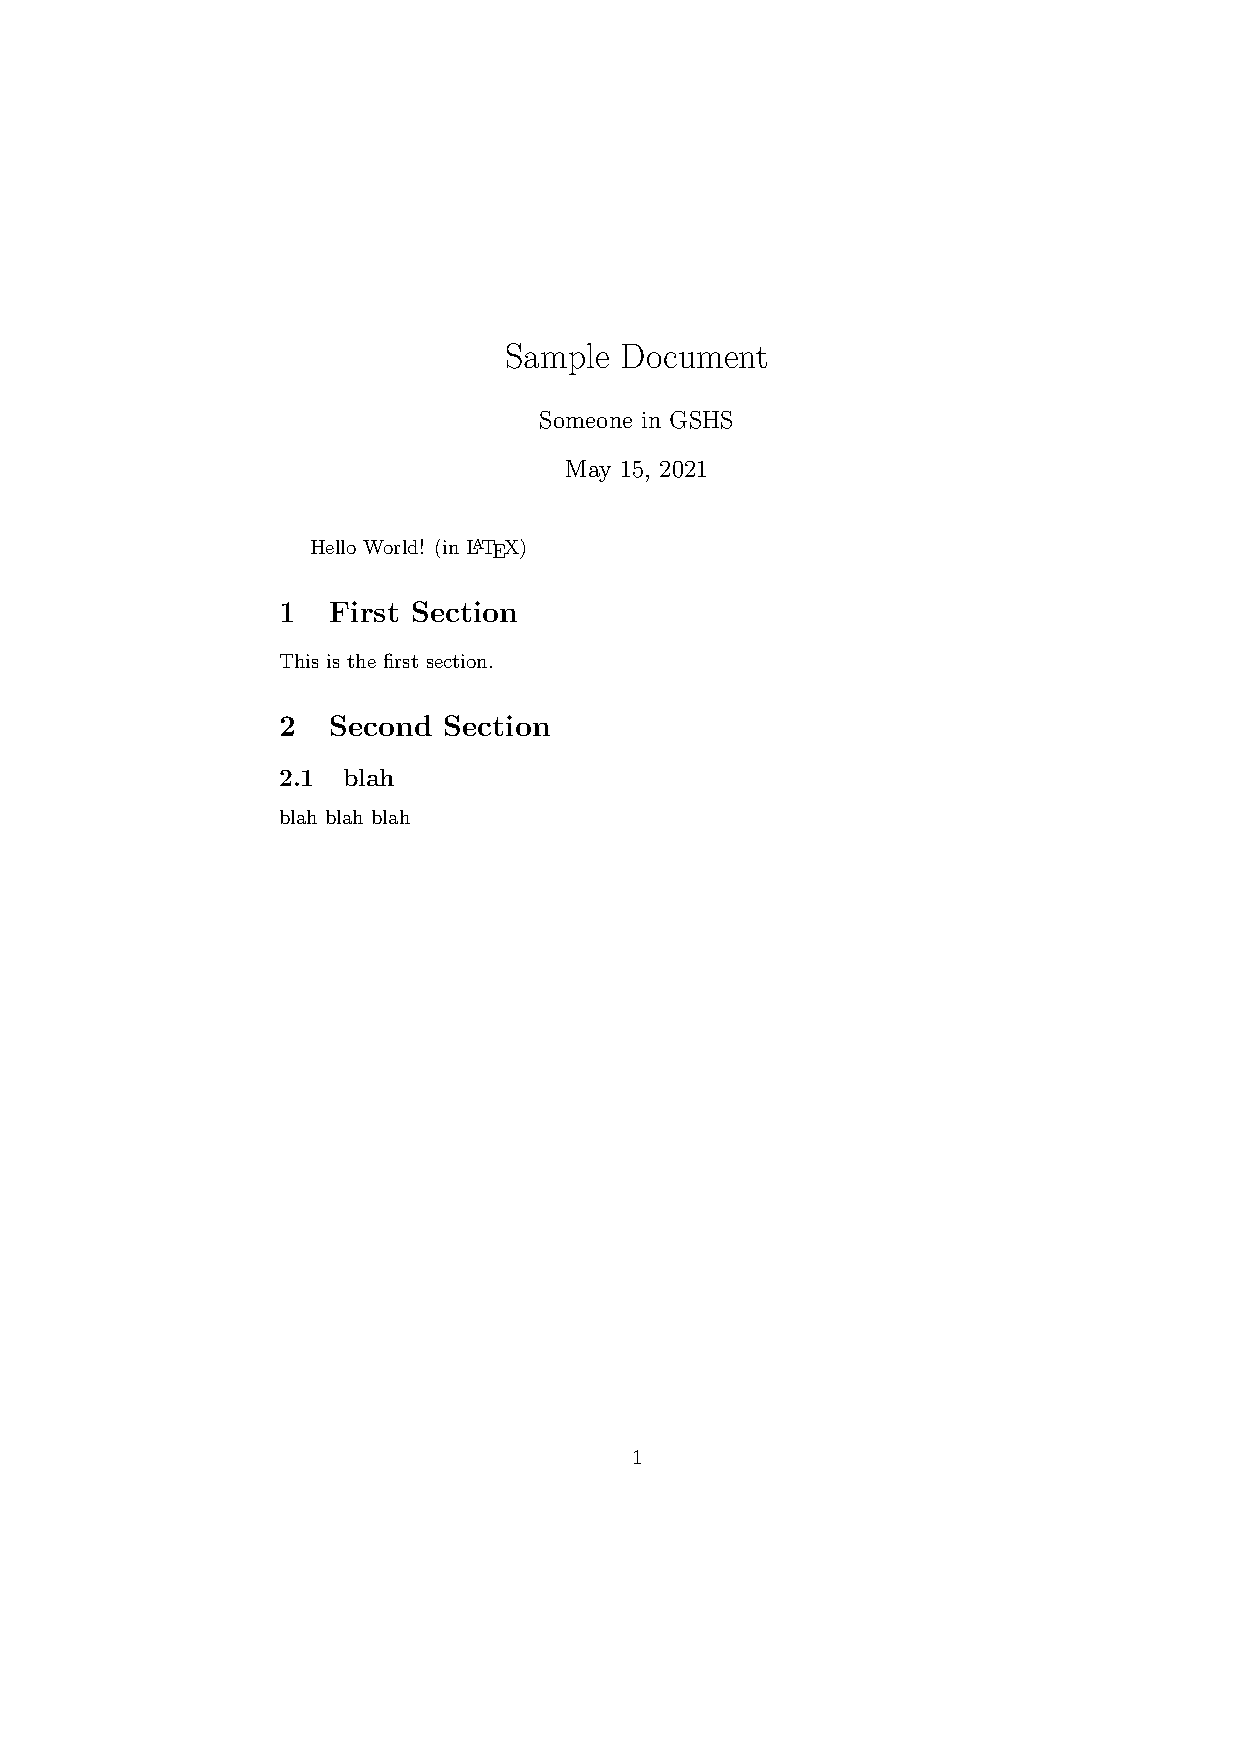
\includegraphics[width=.7\textwidth,trim={4cm 15cm 4cm 5.5cm},clip]{./pdf/ex3.pdf}
	\end{framed}
	
	\LaTeX 은 장절 번호를 자동으로 매겨준다. 예를 들어 1장과 2장 사이에 새로운 장을 추가하면 원래 2장이었던 장은 자동으로 3장이 된다.
	
\end{frame}

\begin{frame}[t, fragile]{목차(ToC, Table of Contents) 만들기}
	\texttt{\tbs tableofcontents}를 사용하면 \LaTeX 에서 자동으로 목차(ToC)를 만들어준다. (ToC는 2번 컴파일해야 제대로 반영된다.)
	
\begin{block}{}
\begin{lstlisting}
(...)
\begin{document}

\maketitle
\tableofcontents

Hello World! (in \LaTeX)

\section{First Section}
This is the first section.

\section{Second Section}
\subsection{blah}
blah blah blah

\end{document}
\end{lstlisting}
\end{block}

\end{frame}

\begin{frame}[t]{목차 만들기}
	
	(컴파일 결과)
	\begin{framed}
		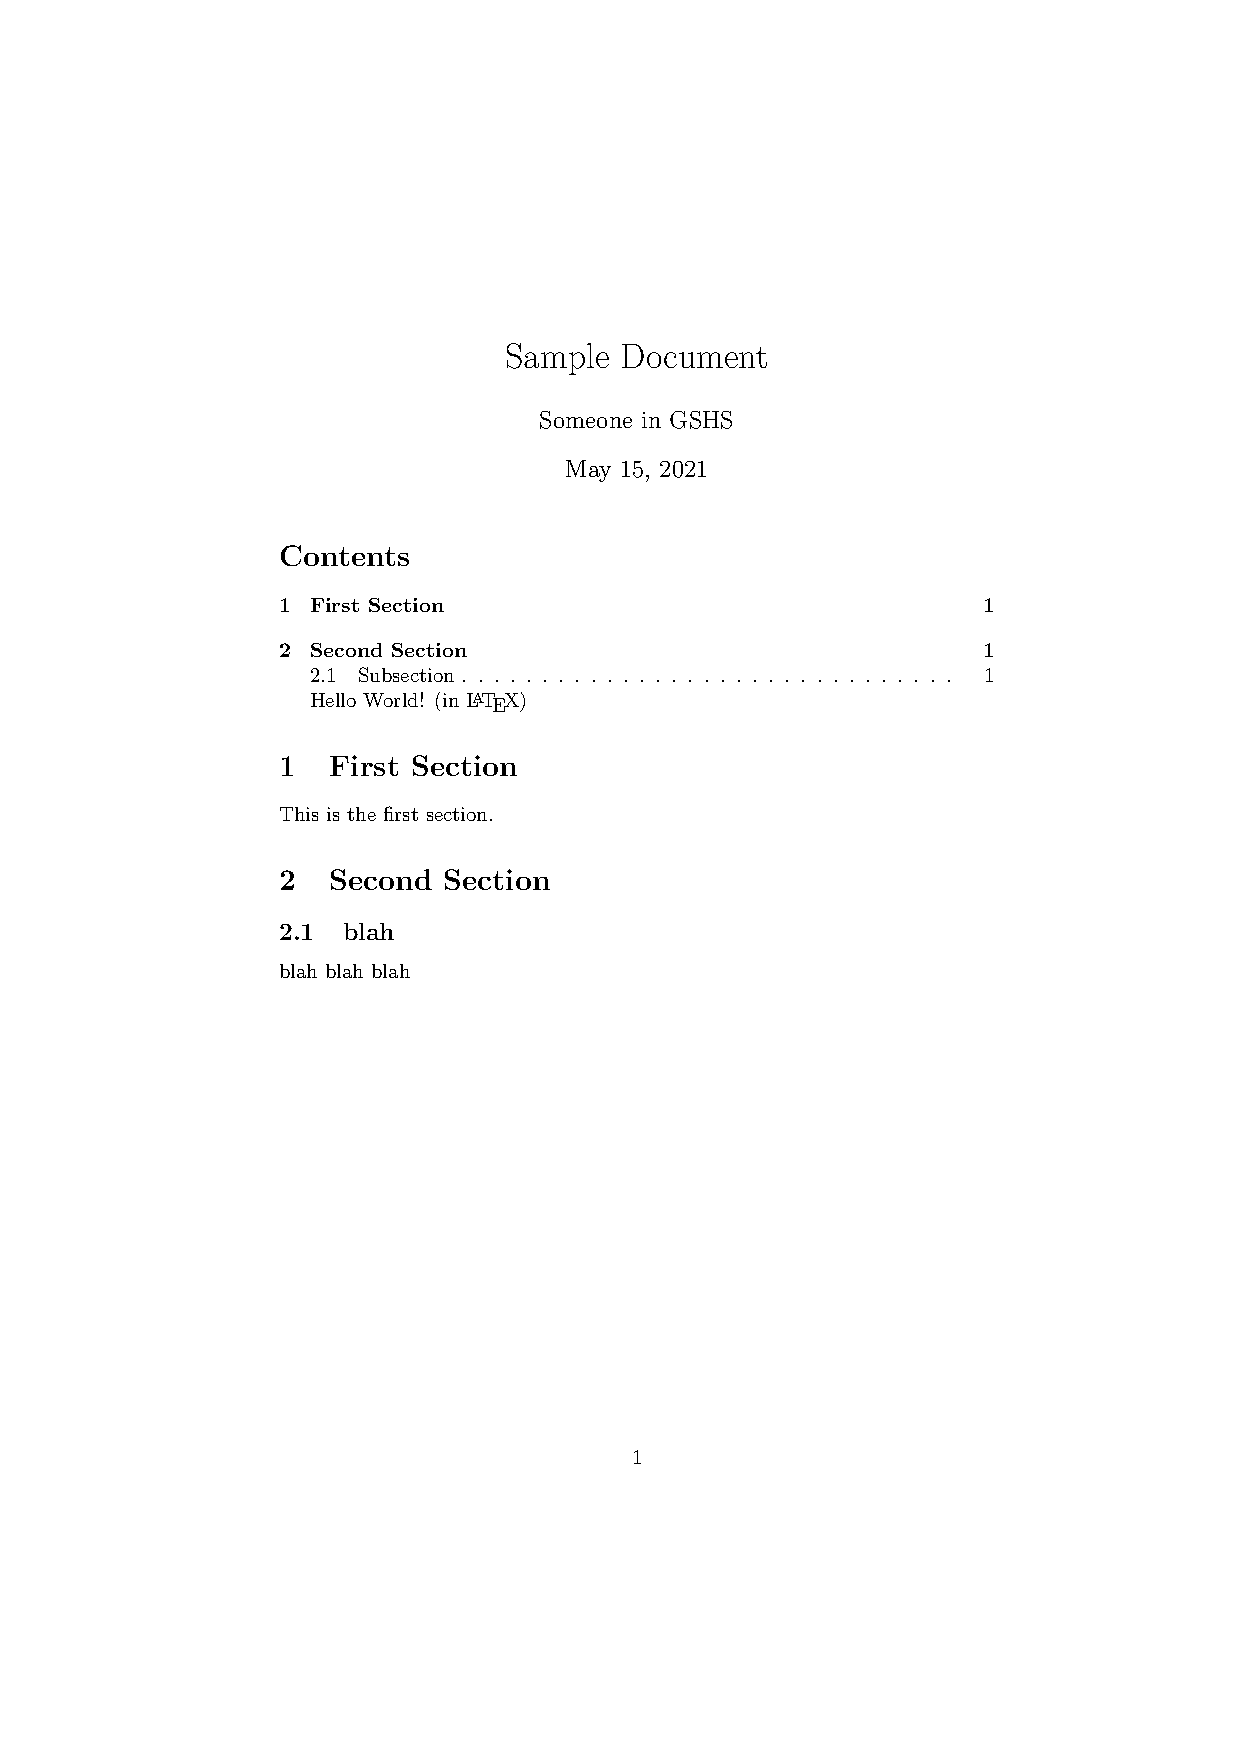
\includegraphics[width=.9\textwidth,trim={4cm 15cm 4cm 5.5cm},clip]{./pdf/ex4.pdf}
	\end{framed}
	
\end{frame}

\begin{frame}[t, fragile]{환경으로 초록 작성하기}
	
	환경(environment)은 \texttt{\tbs begin}으로 시작해 \texttt{\tbs end}로 끝난다. 환경을 통해 초록, 그림, 표 등의 다양한 요소들을 추가할 수 있다. \\
	\vspace{10pt}
	여기서는 \texttt{abstract} 환경을 사용해 초록을 작성해 보자.
	
	
\begin{block}{}
\begin{lstlisting}
(...)
\begin{document}

\maketitle
\tableofcontents

\begin{abstract}
	Short
\end{abstract}

(...)
\end{lstlisting}
\end{block}

\end{frame}

\begin{frame}[t]{환경으로 초록 작성하기}
	
	\begin{framed}
		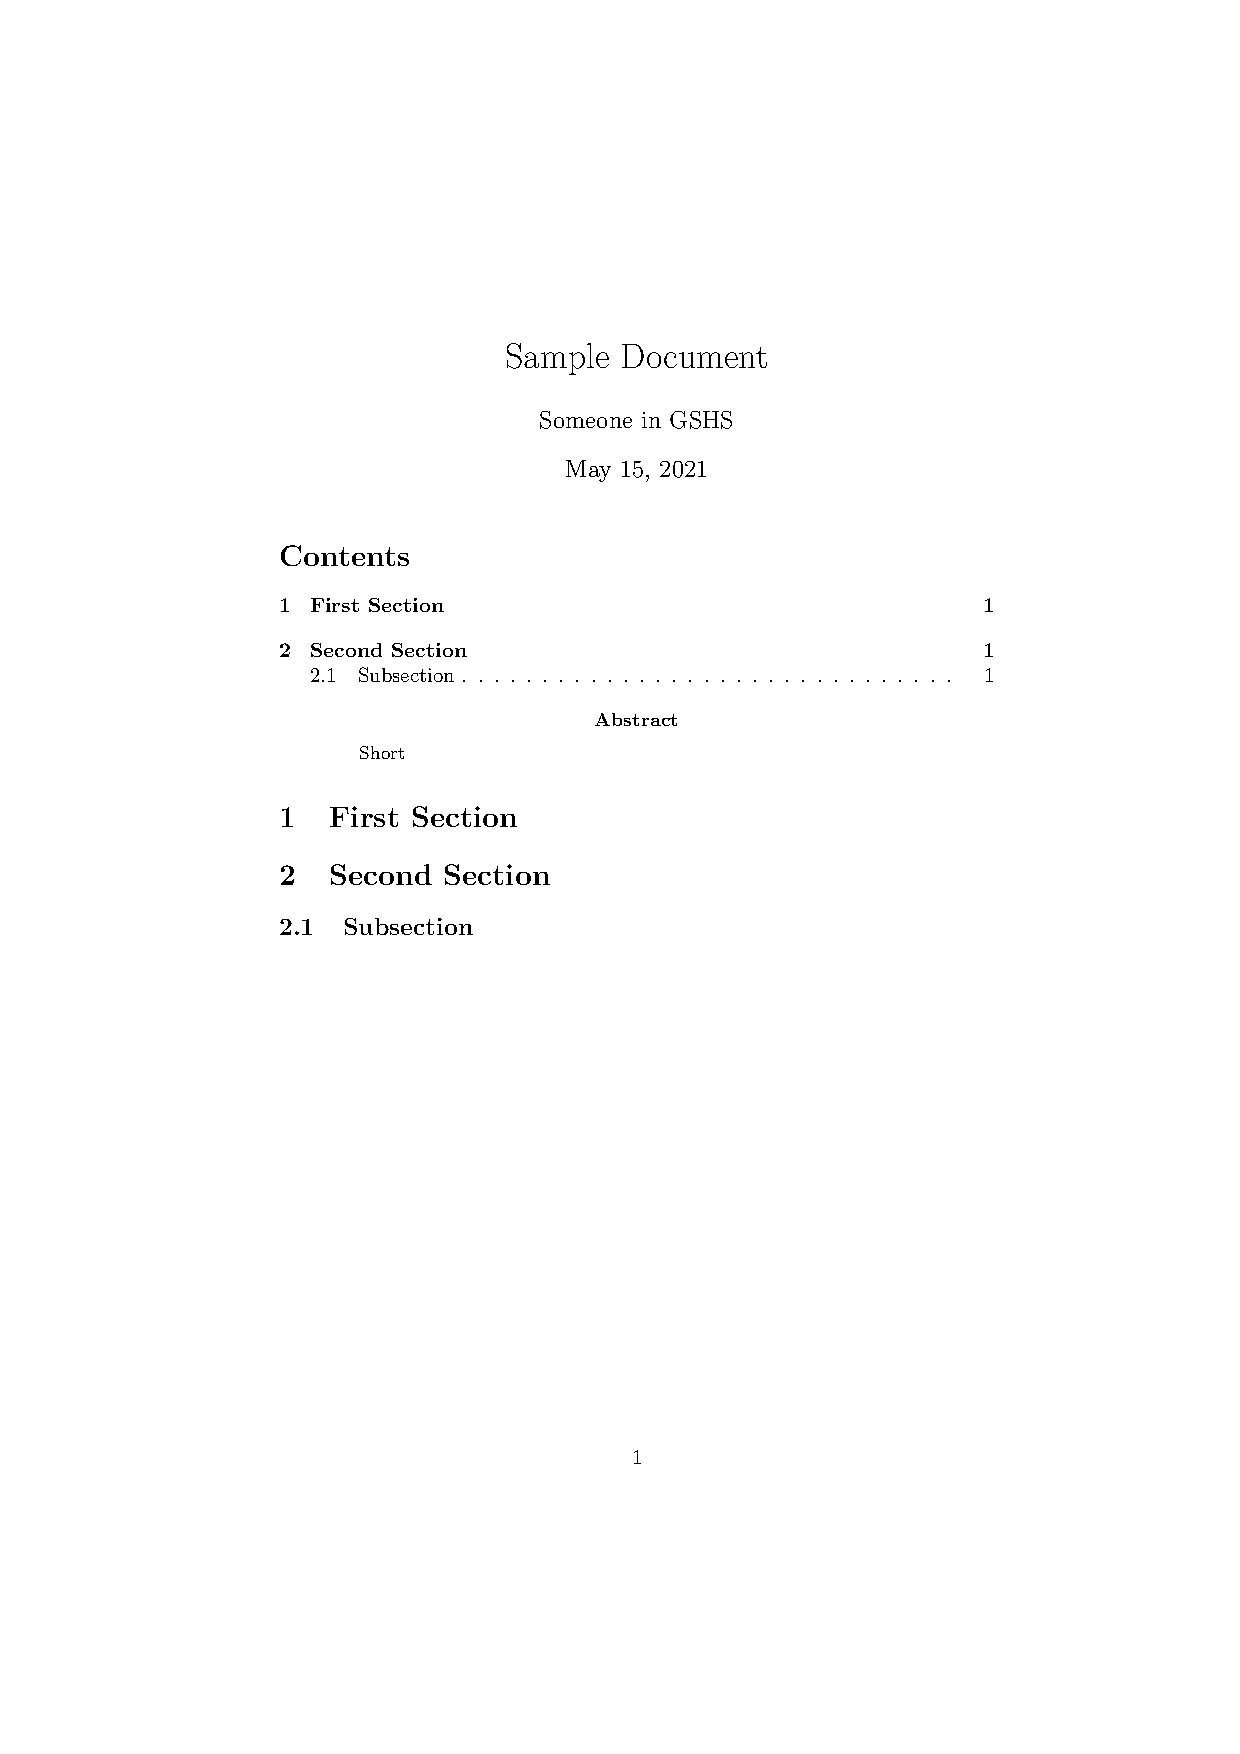
\includegraphics[width=.9\textwidth,trim={4cm 16cm 4cm 5cm},clip]{./pdf/ex5.pdf}
	\end{framed}

\end{frame}



\section{\LaTeX \ Basic}


\begin{frame}[t]{특수문자}
	
	\LaTeX 에서 다음과 같은 특수문자는 바로 사용할 수 없다.
	\begin{center}
		\tbs, \#, \$, \%, \&, \{, \}, \_, \textasciitilde, \textasciiacute
	\end{center}
	다음과 같이 입력해야 한다.
	\begin{center}
		\texttt{\tbs textbackslash, \tbs \#, \tbs \$, \tbs \%, \tbs \&, \tbs \{, \tbs \}, \tbs \_, \tbs textasciitilde, \tbs textasciiacute}
	\end{center}

	특수문자들은 주로 명령어나 환경을 넣을 때 이용된다.
	\begin{itemize}
		\item \$ 는 수식을 넣을 때 이용된다.
		\item \% 는 주석을 넣을 때 이용된다. (Ctrl + T)
	\end{itemize}
	
\end{frame}

\begin{frame}[t]{띄어쓰기}
	
	\begin{itemize}
		\item \LaTeX{}에서는 Space Bar를 아무리 눌러도 1칸만 띄어진다.
		\item 여러 칸 띄어 쓰기 위해서는 `\tbs \ ' (backslash + space bar) 를 사용한다.\\
		\item 이 \tbs \ \ \tbs \ \ \tbs \ \ 렇게 쓰면 이 \ \ \ 렇게 나온다.
		\item \tbs 가 들어간 명령어 뒤에서는 한 칸 띄어야 한다.
		\begin{itemize}
			\item \texttt{\tbs LaTeX를 (X)} $\rightarrow$ \texttt{\tbs LaTeX 를 (O)}
		\end{itemize}
		\item 또는 명령어 뒤에 \{\}를 붙여도 된다.
		\begin{itemize}
			\item \texttt{\tbs LaTeX를 (X)} $\rightarrow$ \texttt{\tbs LaTeX\{\}를 (O)}
		\end{itemize}
	\end{itemize}
	
\end{frame}


\begin{frame}[t]{줄 바꿈}
	
	\begin{itemize}
		\item \tbs \tbs 를 쓰면 줄바꿈이 이루어진다.
		\item 또는 Enter 키를 두 번 눌러도 줄바꿈이 된다. 이때 다음 문장은 들여쓰기가 된다.
		\item 원하는 간격만큼 띄우고 싶다면 \texttt{\tbs vskip 12pt}를 사용한다.\footnote[frame]{pt 대신 pc(=12pt), em(=0.1pt)을 단위로 사용하여도 관계 없다.}
		\item \texttt{\tbs indent}나 \texttt{\tbs noindent}를 문장 앞에서 사용해 들여쓰기를 각각 만들거나 없앨 수 있다.
	\end{itemize}
\end{frame}


\begin{frame}[t, fragile]{따옴표}
	작은따옴표는 \` \ (backtick, Esc키 바로 아래) 과 ' (apostrophe)으로 쓴다.
\begin{block}{}
\textasciigrave 꼭 이기고 말 테야.'
\end{block}
\begin{framed}
	`꼭 이기고 말 테야.'
\end{framed}

	큰따옴표는 이를 2개씩 쓴다.
	
\begin{block}{}
	\textasciigrave\textasciigrave 어, 나가\tbs textasciitilde.''
\end{block}
\begin{framed}
	``어, 나가$\sim$.''
\end{framed}

\end{frame}


\begin{frame}[t, fragile]{좌측, 우측, 중앙 정렬}
	좌측, 우측, 중앙 정렬을 하기 위해서는 각각 \texttt{flushleft, flushright, center} 환경을 사용한다.
	\begin{flushleft}
		좌측 담장
	\end{flushleft}
	\begin{center}
		중앙 담장
	\end{center}
	\begin{flushright}
		우측 담장
	\end{flushright}
	
	\begin{block}{}
		\begin{lstlisting}
\begin{flushleft}
	<@좌측 담장@>
\end{flushleft}
		\end{lstlisting}
	\end{block}
\end{frame}

\begin{frame}[t]{여러 가지 글꼴}
	
	\textbf{글꼴(Font Families)}
	\begin{itemize}
		\item \texttt{\tbs textrm\{ ... \}} : \textrm{Roman, 명조체}
		\item \texttt{\tbs textsf\{ ... \}} : \textsf{Sans serif, 고딕체}
		\item \texttt{\tbs texttt\{ ... \}} : \texttt{Typewriter, 타자기 글꼴}
	\end{itemize}

\vspace{20pt}
\TeX 의 기본 한글 글꼴은 나눔명조와 나눔고딕, 영어 글꼴은 Computer Modern이다. Times New Roman과 같이 더 다양한 글꼴을 사용하려면, 관련 패키지를 사용하면 된다.\footnote[frame]{http://pastebin.com/fZphiXGT}

\end{frame}

\begin{frame}[t]{글꼴 크기}

\textbf{글꼴 크기(Font Size)}
\begin{itemize}
	\item \texttt{\tbs tiny ABCD} : \ \ \ \ \ \ \ \ \ \ \ \ \ \tiny ABCD \small
	\item \texttt{\tbs small ABCD} : \ \ \ \ \ \ \ \ \ \ \  \small ABCD \small
	\item \texttt{\tbs normalsize ABCD} : \ \ \  \normalsize ABCD \ \ \ \ \ (기본값)\small
	\item \texttt{\tbs huge ABCD} : \ \ \ \ \ \ \ \ \ \ \  \ \huge ABCD \small
\end{itemize}

\vskip 1pc
	
	글꼴 크기의 순서는 다음과 같다.
	
	\tiny tiny --- \scriptsize scriptsize --- \footnotesize footnotesize --- \small small --- \normalsize normalsize --- \large large --- \Large Large --- \huge huge --- \Huge Huge \small

\end{frame}

\begin{frame}[t]{글꼴 서식 및 색상}
	
	\textbf{글꼴 서식(Font Series \& Shape)}
	\begin{itemize}
		\item \texttt{\tbs textbf\{ ... \}} : \textrm{\textbf{Boldface}}
		\item \texttt{\tbs textit\{ ... \}} : \textrm{\textit{Italic}}
		\item \texttt{\tbs textsl\{ ... \}} : \textrm{\textsl{Slanted}}
		\item \texttt{\tbs textsc\{ ... \}} : \textrm{\textsc{Small cap}}
	\end{itemize}
	\vspace{20pt}
	
	\textbf{글꼴 색상(Font Color)}
	\begin{itemize}
		\item \texttt{\tbs color\{blue\} ... } : \textrm{\color{blue} This color is blue!}
	\end{itemize}
	
	\texttt{\tbs color}는 color 패키지가 있어야 사용할 수 있다.
	
\end{frame}

\begin{frame}[t, fragile]{목록 만들기}
	목록에는 itemize와 enumerate 환경이 있다. itemize 환경은 순서를 매길 필요가 없는 목록을 만들 때 사용된다.
	
	\vspace{20pt}
	e.g. 경기과학고에 있는 건물들
	\begin{itemize}
		\item 창조관
		\item SRC
		\item 학술정보관
	\end{itemize}
	\begin{block}{}
		\begin{lstlisting}
\begin{itemize}
	\item <@창조관@>
	\item SRC
	\item <@학술정보관@>
\end{itemize}
		\end{lstlisting}
	\end{block}
\end{frame}

\begin{frame}[t, fragile]{목록 만들기}
	enumerate 환경을 사용하면 일련번호가 매겨진다. 실험 과정과 같이 순서가 있는 목록을 만들 때 유용하다.
	
	\vspace{20pt}
	e.g. 평일 아침 우리의 일과
	\begin{enumerate}
		\item 기상 음악을 들으면서 일어난다.
		\item 아침 점호를 받는다.
		\item 급식실에 가서 아침식사를 한다.
	\end{enumerate}
\begin{block}{}
\begin{lstlisting}
\begin{enumerate}
	\item <@기상 음악을 들으면서 일어난다.@>
	\item <@아침 점호를 받는다.@>
	\item <@급식실에 가서 아침식사를 한다.@>
\end{enumerate}		
\end{lstlisting}
\end{block}
\end{frame}

\begin{frame}[t, fragile]{목록 만들기}
	다음의 예시처럼 한 목록 안에 또 하나의 목록을 넣는 것도 가능하다.
	
	\begin{block}{}
		\begin{lstlisting}
\begin{enumerate}
	\item <@1교시@>
	\item <@2교시@>
	\item <@3교시@>
	\item <@4교시@>
	\item <@점심시간@>
	\begin{itemize}
		\item <@주로 12시 50분에 밥을 먹는다.@>
		\item <@4교시가 공강이면 일찍 먹을 수 있다.@>
		\begin{itemize}
			\item <@4교시가 실험 과목이라면 높은 확률로 밥을 늦게 먹는다.@>
		\end{itemize}
	\end{itemize}
\end{enumerate}		
		\end{lstlisting}
	\end{block}
	
\end{frame}



\section{Equations}

\begin{frame}[t, fragile]{수식 넣기 개요}
	문서의 전언에 amsmath 패키지를 불러오자. (다양한 수식 기능 지원)\\
	\begin{block}{}
	\begin{lstlisting}
\usepackage{amsmath}	%in the preamble
	\end{lstlisting}
\end{block}	
\vspace{10pt}
	\textbf{수식을 넣는 3가지 방법}
	\begin{enumerate}
		\item \texttt{\$ ... \$}, \texttt{\tbs ( ... \tbs)} \ \ \ \ \ \ \ \ \ \ \ $\rightarrow$ 행 내(inline)
		\item \texttt{\tbs [ ... \tbs]} \ \ \ \ \ \ \ \ \ \ \ \ \ \ \ \ \ \ \ \ \ \ \ $\rightarrow$ 표시형(displaystyle)
		\item equation, align, gather 환경 \ \ $\rightarrow$ 표시형(displaystyle)
	\end{enumerate}
\end{frame}

\begin{frame}[t, fragile]{기본 수식 기호}
	\begin{enumerate}
		\item 덧셈과 뺄셈: +, -, \texttt{\tbs pm}
		\item 곱셈: \texttt{\textbackslash times}
		\item 분수: \texttt{\tbs frac}\{분자\}\{분모\}
		\item 위첨자: \{밑\}\^ \ \{위첨자\}
		\item 아래첨자: \{수식\}\_\{아래첨자\}
		\item 그리스 문자
		\begin{itemize}
			\item 소문자: \texttt{\tbs alpha, beta,} $\cdots$
			\item 대문자: \texttt{\tbs Alpha, Beta,} $\cdots$
		\end{itemize}
		\item 벡터: \texttt{\tbs vec}\{내용\}, \texttt{\tbs mathbf}\{내용\}
		\item 합(\texttt{sum})과 적분(\texttt{int}): \texttt{\tbs int}\_\{아래끝\}\^ \ \{위끝\}
		\item 그 외 모르는 것은 검색. 하다보면 외워진다!
	\end{enumerate}
	
\end{frame}

\begin{frame}[t, fragile]{수식 넣기 --- 행 내 수식}
	
	\textbf{\texttt{\$ ... \$} 또는 \texttt{\tbs ( ... \tbs)} 이용} : 행 내(inline) 수식
	
	\vspace{10pt}
	
$ 1 + 2 = 3 $ \\
$ f(x) = \frac{1}{x} $입니다. \\
$ e^{i\pi} + 1 = 0 $ \\
$ \sqrt{4} = \sqrt[3]{8} = 2 $ \\
	
\begin{block}{}
	\begin{lstlisting}
$ 1 + 2 = 3 $ \\
$ f(x) = \frac{1}{x} $<@입니다.@> \\
$ e^{i\pi} + 1 = 0 $ \\
$ \sqrt{4} = \sqrt[3]{8} = 2 $ \\

% \( ... \)<@으로 바꾸어 넣어도 동일@>
	\end{lstlisting}
\end{block}	

행 내 수식은 본문과 수식을 한 줄에 이어쓸 수 있다.
\end{frame}

\begin{frame}[t, fragile]{수식 넣기 --- 표시형 수식}
	
	\textbf{\texttt{\tbs [ ... \tbs]} 이용} : 표시형(displaystyle) 수식

	
	\[ 1 + 2 = 3 \]
	\[ f(x) = \frac{1}{x} \]
	\[ e^{i\pi} + 1 = 0 \]
	\[ \sqrt{4} = \sqrt[3]{8} = 2 \]
	
	\begin{block}{}
		\begin{lstlisting}
\[ 1 + 2 = 3 \]
\[ f(x) = \frac{1}{x} \]
\[ e^{i\pi} + 1 = 0 \]
\[ \sqrt{4} = \sqrt[3]{8} = 2 \]
		\end{lstlisting}
	\end{block}	
	
표시형 수식은 단독으로 한 줄을 차지하고, 가운데 정렬된다.
\end{frame}

\begin{frame}[t, fragile]{Inline vs. Displaystyle}
	
	같은 수식이라도 나타나는 형식이 다른 경우가 있다.

\begin{block}{}
	\begin{lstlisting}
$ \sum_{k=1}^{3} \frac{1}{k} = \frac{11}{6} $
\[ \sum_{k=1}^{3} \frac{1}{k} = \frac{11}{6} \]
	\end{lstlisting}
\end{block}
\begin{itemize}
	\item 행 내 : $\sum_{k=1}^{3} \frac{1}{k} = \frac{11}{6}$
	\item 표시형: $\displaystyle \sum_{k=1}^{3} \frac{1}{k} = \frac{11}{6}$
\end{itemize}

\begin{block}{}
	\begin{lstlisting}
$ \lim_{x \rightarrow 1} \frac{1}{x} $
\[ \lim_{x \rightarrow 1} \frac{1}{x} \]
	\end{lstlisting}
\end{block}
\begin{itemize}
	\item 행 내 : $ \lim_{x \rightarrow 1} \frac{1}{x} $
	\item 표시형: $ \displaystyle \lim_{x \rightarrow 1} \frac{1}{x} $
\end{itemize}

\end{frame}

\begin{frame}[t, fragile]{Inline vs. Displaystyle}
	
	\textbf{Q.} 행 내 수식을 표시형 수식처럼 쓰고 싶어요!
	%\vspace{10pt}
	\begin{itemize}
		\item 따라서 답은 $\sum_{k=1}^{3} \frac{1}{k} = \frac{11}{6}$이다. (X) \ \ \ \ \ \textcolor{magenta!70}{$\leftarrow$ 이렇게 말고...}
		\item 따라서 답은 $\displaystyle \sum_{k=1}^{3} \frac{1}{k} = \frac{11}{6}$이다. (O) \ \ \ \ \ \ \  \textcolor{cyan!70}{$\leftarrow$ 이렇게요!}
	\end{itemize}
	
	\vspace{10pt}
	
	\textbf{A.} 행 내 수식의 시작점에 \texttt{\tbs displaystyle}을 붙이면 됩니다.
	
	\begin{block}{}
		\begin{lstlisting}
<@따라서 답은@> $\displaystyle \sum_{k=1}^{3} \frac{1}{k} = \frac{11}{6}$<@이다.@>
		\end{lstlisting}
	\end{block}
	
	\vspace{7pt}
	(컴파일 결과)
	\vspace{-7pt}
	\begin{framed}
		따라서 답은 $\displaystyle \sum_{k=1}^{3} \frac{1}{k} = \frac{11}{6}$이다.
	\end{framed}
	
\end{frame}

\begin{frame}[t, fragile]{수식 예제}
	
	표시형(displaystyle) 수식을 이용해 작성해보자.
	
\[ z=x+yi \Rightarrow \bar{z}=x-yi ~ (x,y\in\mathbb{R}) \]
\[ \int_{1} ^{\infty} \frac{1}{r^2}dr = \left[ - \frac{1}{r} \right]_{1}^{\infty} = 1 \]
\[ \hat{H} = -\frac{\hbar^2}{2m}\frac{\partial^2}{\partial x^2} + V \]

	\begin{block}{}
		\begin{lstlisting}
\[ z=x+yi \Rightarrow \bar{z}=x-yi ~ (x,y\in\mathbb{R}) \]
\[ \int_{1} ^{\infty} \frac{1}{r^2}dr = \left[ - \frac{1}{r} \right]_{1}^{\infty} = 1 \]
\[ \hat{H} = -\frac{\hbar^2}{2m}
		\frac{\partial^2}{\partial x^2} + V \]
		\end{lstlisting}
	\end{block}	
	
\end{frame}

\begin{frame}[t]{환경을 이용한 수식}
	equation, align, gather 모두 번호가 매겨지고, 표시형 수식이다.
	\begin{itemize}
		\item equation - 단일 행
		\item align - 여러 행, 기준 정렬
		\item gather - 여러 행, 가운데 정렬
	\end{itemize}
	\vskip 1pc
	\begin{itemize}
		\item \texttt{\tbs label}을 사용해 수식에 label을 붙인 후, \texttt{\tbs ref} 또는 \texttt{\tbs eqref}를 통해 참조할 수 있다.
		\item 각 환경에 *을 붙이면 번호가 사라진다.
	\end{itemize}	
\end{frame}

\begin{frame}[t, fragile]{수식 환경 (1) --- equation}
	\begin{equation}
		\Delta \lambda = \frac{h}{mc} (1-\cos\phi)
		\label{eq:compton}
	\end{equation}
	Compton 산란 공식은 식 \eqref{eq:compton}과 같다.

\vspace{10pt}
\begin{block}{equation 환경: 단일 행}
	\begin{lstlisting}
\begin{equation}
	\Delta\lambda = \frac{h}{mc} (1-\cos\phi)
	\label{eq:compton}
\end{equation}
Compton <@산란 공식은 식@> \eqref{eq:compton}<@과 같다.@>
	\end{lstlisting}
\end{block}	

\vspace{10pt}

	참조를 위해 붙이는 label은 사용하기 쉽도록 붙이는 것이 좋다. 단, label은 알파벳, 숫자, 기호로만 구성되어야 한다. (한글 사용 X)
\end{frame}



\begin{frame}[t, fragile]{수식 환경 (2) --- align}
	등호를 기준으로 정렬한 수식
	\begin{align*}
		(a+b)^2 &= (a+b)(a+b)\\
		&= a^2 + ab + ba + b^2\\
		&= a^2 + 2ab + b^2
	\end{align*}

\begin{block}{align 환경: 정렬 위치 지정}
	\begin{lstlisting}
\begin{align*}
	(a+b)^2 &= (a+b)(a+b) \\
	&= a^2 + ab + ba + b^2 \\
	&= a^2 + 2ab + b^2
\end{align*}
	\end{lstlisting}
\end{block}	

\vspace{10pt}

	행의 구분은 \tbs \tbs 로 하고, 각 행에서 정렬 위치에 \&를 붙인다. 위 코드애서 기준 위치는 등호이다.

\end{frame}

\begin{frame}[t, fragile]{수식 환경 (3) --- gather}
	
	\begin{gather}
		a + b + c = 6 \\
		2a + b + c = 8 \\
		2a + 2b + c = 13
	\end{gather}
	
	\begin{block}{gather 환경}
		\begin{lstlisting}
\begin{gather}
	a + b + c = 6 \\
	2a + b + c = 8 \\
	2a + 2b + c = 13
\end{gather}
		\end{lstlisting}
	\end{block}	
	
	\vspace{10pt}
	
	행의 구분은 \tbs \tbs 로 하며, 모든 행이 가운데 정렬된다.
	
\end{frame}


\begin{frame}[t, fragile]{수식 글꼴}
	
	\textbf{여러 가지 수식 글꼴}
	\begin{itemize}
		\item \texttt{\$\tbs mathcal\{ABCDEFGH\}\$} : $\mathcal{ABCDEFGH}$ (흘림체, calligraphic)
		\item \texttt{\$\tbs mathfrak\{ABCDEFGH\}\$} : $\mathfrak{ABCDEFGH}$ (프락투어, fraktur)
		\item \texttt{\$\tbs mathbb\{ABCDEFGH\}\$} : $\mathbb{ABCDEFGH}$ (칠판볼드체, blackboard)
	\end{itemize}
	
	\textbf{스크립트 글꼴}
	
	Ralph Smith's Formal Script Font을 불러오기 위해 \texttt{mathrsfs} 패키지를 불러온다.
	\begin{block}{}
		\begin{lstlisting}
\usepackage{mathrsfs}	%in the preamble
		\end{lstlisting}
	\end{block}
	\begin{itemize}
		\item \texttt{\$\tbs mathscr\{ABCDEFGH\}\$} : $\mathscr{ABCDEFGH}$
	\end{itemize}
	
\end{frame}

\begin{frame}[t, fragile]{수식 예제 --- Adv}
	
	gather* 환경을 이용해 작성해보자.
\begin{gather*}
[T]_\mathcal{C} = P^{-1} [T]_\mathcal{B} P \\
\mathfrak{I}(z) = \frac{z - \bar{z}}{2i} \\
\mathscr{P} \subset \mathscr{D} \subset \mathscr{C} \subset \mathscr{F}
\end{gather*}
	
	\begin{block}{}
		\begin{lstlisting}
\begin{gather*}
	[T]_\mathcal{C} = P^{-1} [T]_\mathcal{B} P \\
	\mathfrak{I}(z) = \frac{z - \bar{z}}{2i} \\
	\mathscr{P} \subset \mathscr{D} \subset \mathscr{C} \subset \mathscr{F}
\end{gather*}
		\end{lstlisting}
	\end{block}	
	
\end{frame}


\begin{frame}[t, fragile]{수식 정리}
	
	
	\begin{itemize}
		\item 행 내: \textbf{\texttt{\$ ... \$}} \\ $\rightarrow$ 표시형처럼 쓰려면 수식 처음에 \texttt{\tbs displaystyle} 입력
		\item 표시형 (행 1개): \textbf{equation 환경} \\ $\rightarrow$ 번호 불필요시 equation* 환경 또는 \tbs[ ... \tbs]
		\item 표시형 (행 여러 개): \textbf{align 환경} \\ $\rightarrow$ \tbs \tbs 로 행 바꿈, \& 기호로 정렬 위치 조정
		
	\end{itemize}

\vspace{20pt}

	\LaTeX 의 수식 입력 방식이 다양해서 처음에는 복잡해 보이지만, 쓰다보면 주요한 몇 가지 위주로 사용하게 될 것이다. 계속 쓰면서 익숙해지면 알겠지만 \LaTeX 은 그 어떤 수식 편집기보다도 다루기가 편리하고, 결과물 수식도 꽤나 아름답다!
	
\end{frame}


\section{Figures \& Tables}

\subsection{Figures}
\begin{frame}[t, fragile]{그림 불러오기}

	그림을 불러오기 위해서는 graphicx 패키지가 필요하다.
	
\begin{block}{}
\begin{lstlisting}
\usepackage{graphicx}	% in the preamble
\end{lstlisting}
\end{block}	

	이제 그림을 넣기 위한 사전 작업을 하자.
	\begin{itemize}
		\item 일단 그림 파일 하나를 마련하자.
		\item 파일명은 알파벳과 숫자만으로 구성하자.
		\item 그 그림을 *.tex 파일과 같은 폴더에 넣자.
	\end{itemize}

\end{frame}

\begin{frame}[t, fragile]{그림 불러오기}
	
	그림의 경로가 `./figures/gshs.jpg'일 때, 문서의 본문에 이렇게 입력하자.
	
	
\begin{block}{}
	\begin{lstlisting}

\includegraphics[width=.2\textwidth]{./figures/gshs.jpg}
	\end{lstlisting}
\end{block}	

\vspace{10pt}
(컴파일 결과)
\vspace{-10pt}
\begin{framed}

\includegraphics[width=.2\textwidth]{./figures/gshs.jpg}
\end{framed}

\end{frame}

\begin{frame}[t, fragile]{Figure 환경 이용하기}
	
	보고서를 작성할 때는 그림에 번호와 캡션을 달아야 한다. \texttt{figure} 환경으로 번호와 캡션을 달 수 있다. 환경 안에 다음 세 명령어를 넣는다. \\
	$\rightarrow$ \tbs\texttt{includegraphics}, \tbs\texttt{caption}, \tbs\texttt{label}
	\vspace{10pt}
	
	라벨링한 그림은 \tbs\texttt{ref}로 참조한다.
\end{frame}

\begin{frame}[t, fragile]{Figure 환경 이용하기}
	
\vspace{-10pt}
\begin{block}{}
	\begin{lstlisting}
\begin{figure}[h]
    \centering
    
\includegraphics[width=.2\textwidth]{./figures/gshs.jpg}
    \caption{<@경기과학고 로고@>}
    \label{fig:gshs}
\end{figure}
<@그림@> \ref{fig:gshs}<@은 경기과학고의 로고이다.@>
	\end{lstlisting}
\end{block}	

\vspace{3pt}
(컴파일 결과)
\vspace{-5pt}
\begin{framed}
	
\includegraphics[width=\textwidth,trim={4cm 19.3cm 4cm 4.3cm},clip]{practice.pdf}
\end{framed}
\end{frame}

\begin{frame}[t, fragile]{Figure 환경 옵션}

\vspace{-5pt}
\begin{itemize}
	\item figure의 위치: \tbs \texttt{begin\{figure\}} 뒤의 대괄호에 지정
\end{itemize}
\vspace{-10pt}
	\begin{table}[h]
		\centering
		\begin{tabular}{|c|p{0.8\textwidth}|}
			\hline
			h & 코드의 위치(\textbf{h}ere)                                    \\ \hline
			t & 페이지 위(\textbf{t}op)                                      \\ \hline
			b & 페이지 아래(\textbf{b}ottom)                                 \\ \hline
			p & 특정 페이지(\textbf{p}age) (대체로 문서의 맨 뒤)                        \\ \hline
			%! & \LaTeX{}에서 설정한 서식을 무시. (텍스트 여백 등) \\ \hline
		\end{tabular}
	\end{table}
\begin{itemize}
	\item Figure 1: $\rightarrow$ 그림 1:
\end{itemize}
\vspace{-10pt}
\begin{block}{}
	\begin{lstlisting}
\renewcommand{\figurename}{<@그림@>}	%in the preamble
	\end{lstlisting}
\end{block}	

\begin{itemize}
	\item 그림 1: $\rightarrow$ 그림 1.
\end{itemize}
\vspace{-10pt}
\begin{block}{}
	\begin{lstlisting}
\usepackage[labelsep=period]{caption}	%in the preamble
	\end{lstlisting}
\end{block}	

\end{frame}


\subsection{Subfigures}
\begin{frame}[t, fragile]{Subfigure 넣기}

figure 환경 안에 여러 이미지를 넣으려면 subfigure 패키지를 불러와야 한다.
	\begin{block}{}
		\begin{lstlisting}
\usepackage{subfigure}	%in the preamble
		\end{lstlisting}
	\end{block}	

본문에 새로운 figure 환경을 만들어 subfigure을 써보자.
\begin{block}{}
	\begin{lstlisting}
\begin{figure}[h]
	\centering
	\subfigure[h][Bears]{
\includegraphics[width=.2\textwidth]{./figures/bears.jpg}}
	\subfigure[h][Twins]{
\includegraphics[width=.2\textwidth]{./figures/twins.png}}
	\caption{Baseball Teams in Jamsil}
	\label{fig:jamsil}
\end{figure}
<@그림@> \ref{fig:jamsil}<@는 잠실 야구장을 홈으로 쓰는 프로야구 구단들이다.@>
	\end{lstlisting}
\end{block}

\end{frame}


\begin{frame}[t, fragile]{Subfigure 넣기}
	
(컴파일 결과)
\vspace{-10pt}
\begin{framed}
	
\includegraphics[width=\textwidth,trim={4cm 19cm 4cm 4.3cm},clip]{practice2.pdf}
\end{framed}

	
\end{frame}


\subsection{Tables}
\begin{frame}[t, fragile]{표 넣기}
\LaTeX \ 표를 만드는 명령어는 매우 비효율적이다. `LaTeX Table Generator'를 사용하는 것을 추천한다.

%\vspace{20pt}

\begin{itemize}
	\item 사이트: \url{https://www.tablesgenerator.com/}
	\item 이용 방법: 사이트 접속 $\rightarrow$ 표 채우기 $\rightarrow$ Generate $\rightarrow$ Copy to Clipboard $\rightarrow$ \LaTeX \ 코드에 붙여넣기
\end{itemize}

\end{frame}

\begin{frame}[t, fragile]{표 넣기}
table 환경 내의 tabular 환경에서 표를 만들 수 있다.

\begin{block}{}
	\begin{lstlisting}
\begin{table}[h]
	\begin{tabular}{|c|l|}
		\hline
		<@SRC@> & <@본관에서 제일 멀다@> \\ \hline
		<@학습관@> & <@2, 3학년 학습실@> \\ \hline
		<@아름관@> & <@최고 해발고도@> \\ \hline
	\end{tabular}
\end{table}
	\end{lstlisting}
\end{block}

(컴파일 결과)
\vspace{-10pt}
\begin{framed}
	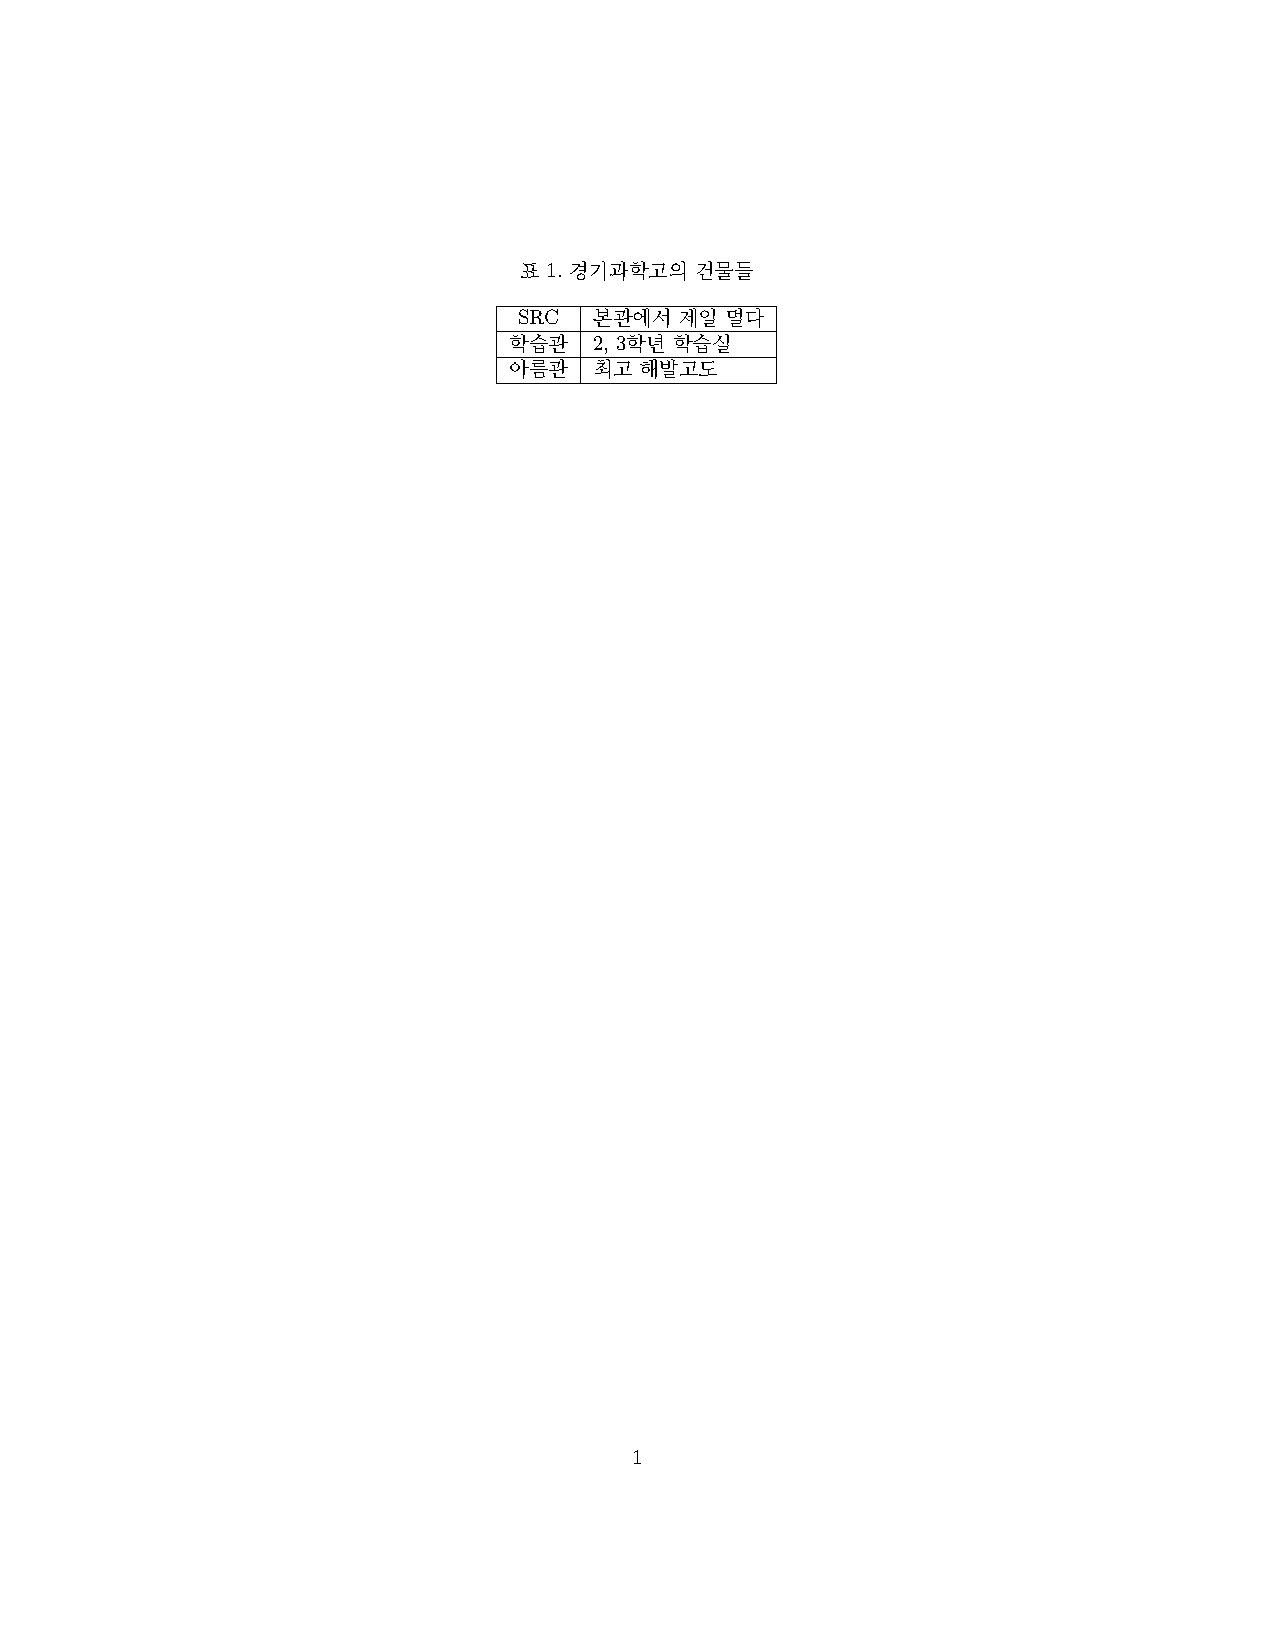
\includegraphics[width=\textwidth,trim={4cm 21.3cm 4cm 5cm},clip]{./pdf/table1.pdf}
\end{framed}

\end{frame}

\begin{frame}[t, fragile]{표 넣기}
	\begin{itemize}
		\item 캡션과 label 지정
	\end{itemize}
	\vspace{-4pt}
	\begin{block}{}
		\begin{lstlisting}
\begin{table}[h]
	\caption{<@경기과학고의 건물들@>}
	\label{tab:gshs_bldgs}
	\begin{tabular}{|c|l|}
		\hline
		<@SRC@> & <@본관에서 제일 멀다@> \\ \hline
		<@학습관@> & <@2, 3학년 학습실@> \\ \hline
		<@아름관@> & <@최고 해발고도@> \\ \hline
	\end{tabular}
\end{table}
		\end{lstlisting}
	\end{block}
	
	\begin{itemize}
		\item Table 1. $\rightarrow$ 표 1.
	\end{itemize}
	\vspace{-4pt}
	\begin{block}{}
		\begin{lstlisting}
\renewcommand{\tablename}{<@표@>}		%in the preamble
		\end{lstlisting}
	\end{block}	
	
\end{frame}


\begin{frame}[t, fragile]{표 넣기}
	
	(컴파일 결과)
	\vspace{-10pt}
	\begin{framed}
		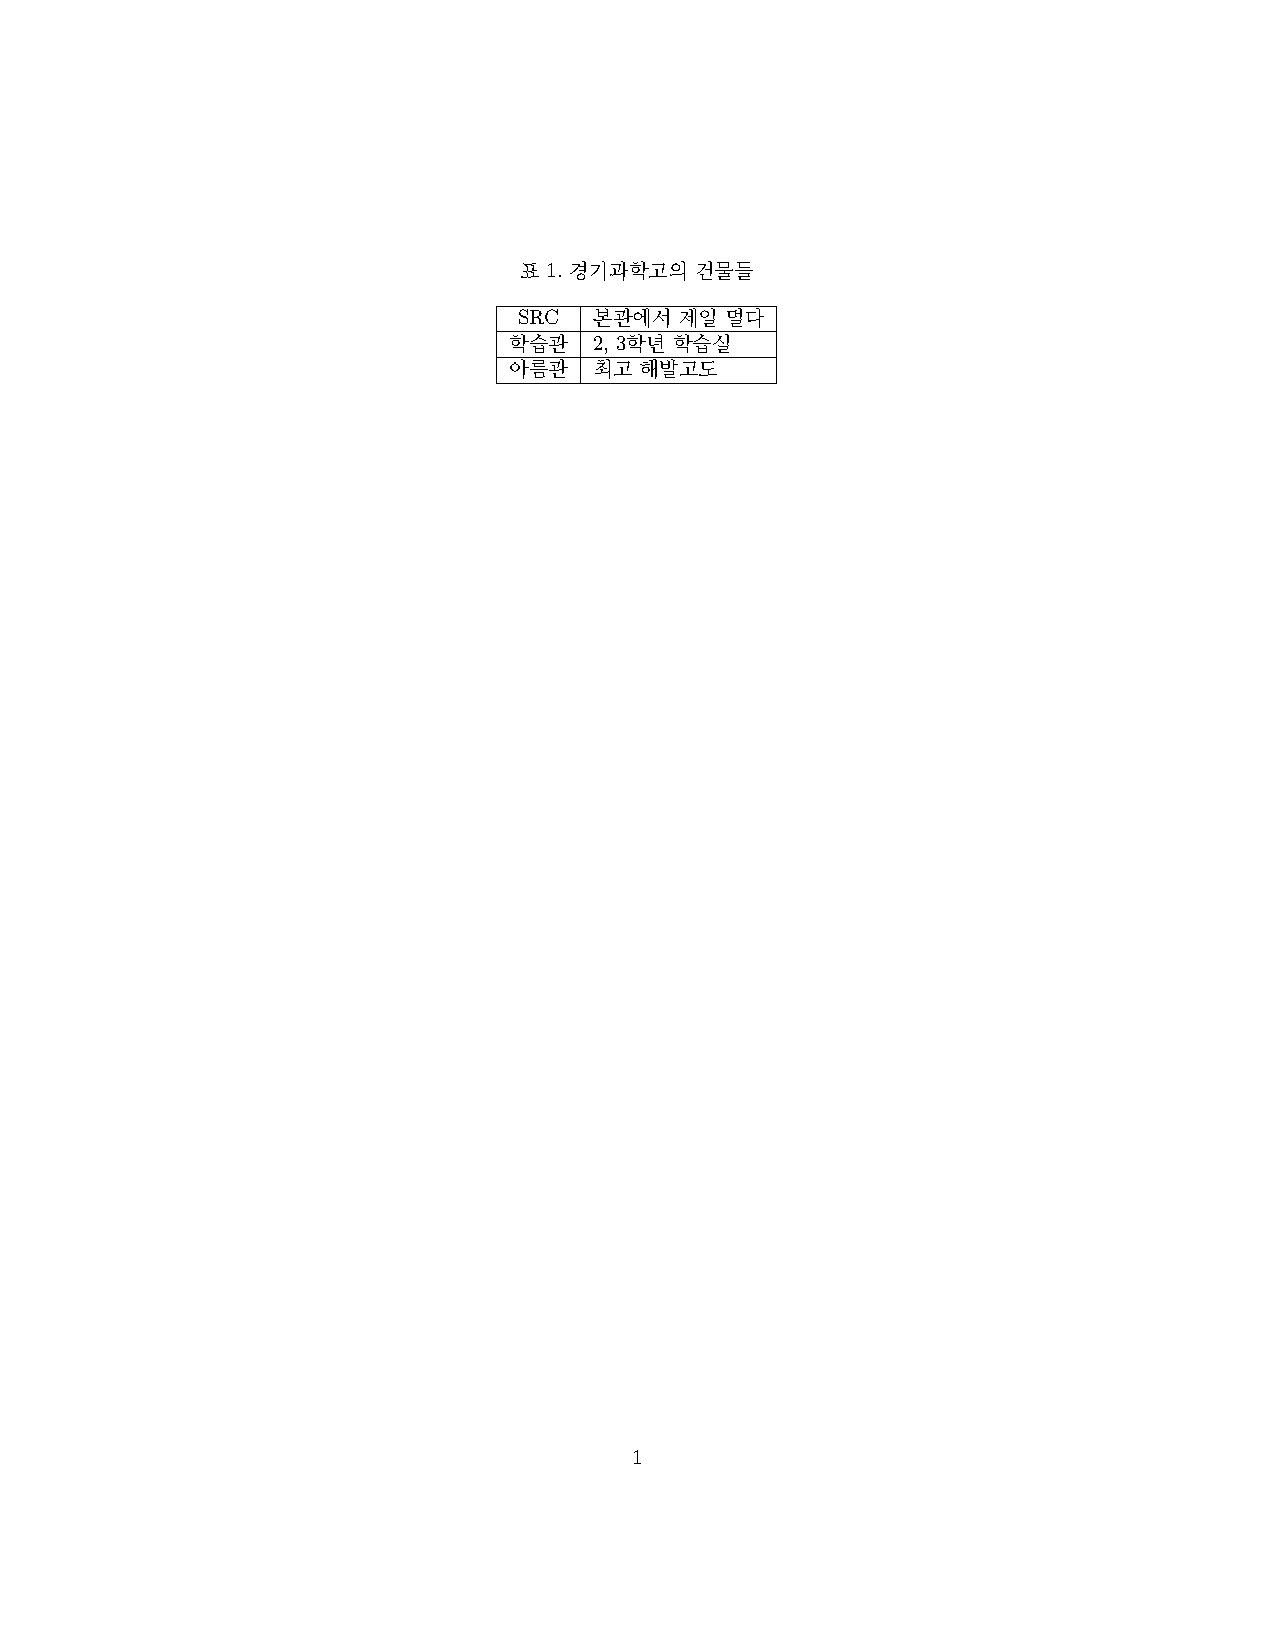
\includegraphics[width=\textwidth,trim={4cm 21cm 4cm 4cm},clip]{./pdf/table1.pdf}
	\end{framed}
	
	
\end{frame}

\section{Referencing \& Citing}

\subsection{Referencing}
\begin{frame}[t]{개체 참조}
	
	\begin{itemize}
		\item \LaTeX 에서는 태그를 통해 참조(reference)가 이루어진다.
		\item label이 붙은 수식, 그림, 표는 번호가 자동으로 매겨진다.
		\item 이때 label은 영어, 숫자, 기호로 구성한다. (한글 사용 X)
\end{itemize}
	
\begin{framed}
	\centering
	\textbackslash \texttt{label\{...\}} $\leftrightarrow$ \textbackslash \texttt{ref\{...\}} \\
\end{framed}
\begin{itemize}
\item 수식: \textbackslash \texttt{eqref\{...\}}
\\ e.g. \textbackslash \texttt{eqref\{eq:compton\}} $\xrightarrow[]{\text{~compile~}}$ \eqref{eq:compton}
\item 그림, 표, 장절: \textbackslash \texttt{ref\{...\}}
\\ e.g. \textbackslash \texttt{ref\{tab:gshs\_bldgs\}} $\xrightarrow[]{\text{~compile~}}$ 1

\end{itemize}
\end{frame}


\subsection{Citing}

\begin{frame}[t, fragile]{참고문헌 목록}
	\begin{itemize}
		\item \LaTeX{}에서는 참고문헌도 자동으로 정리해준다.
		\item 참고문헌 정리 방법에는 \texttt{thebibliography} 환경을 사용하는 방법과 Bib\TeX 을 사용하는 방법이 있다.
		\item 이번에는 \texttt{thebibliography}를 사용해보자.
	\end{itemize}
\begin{framed}
	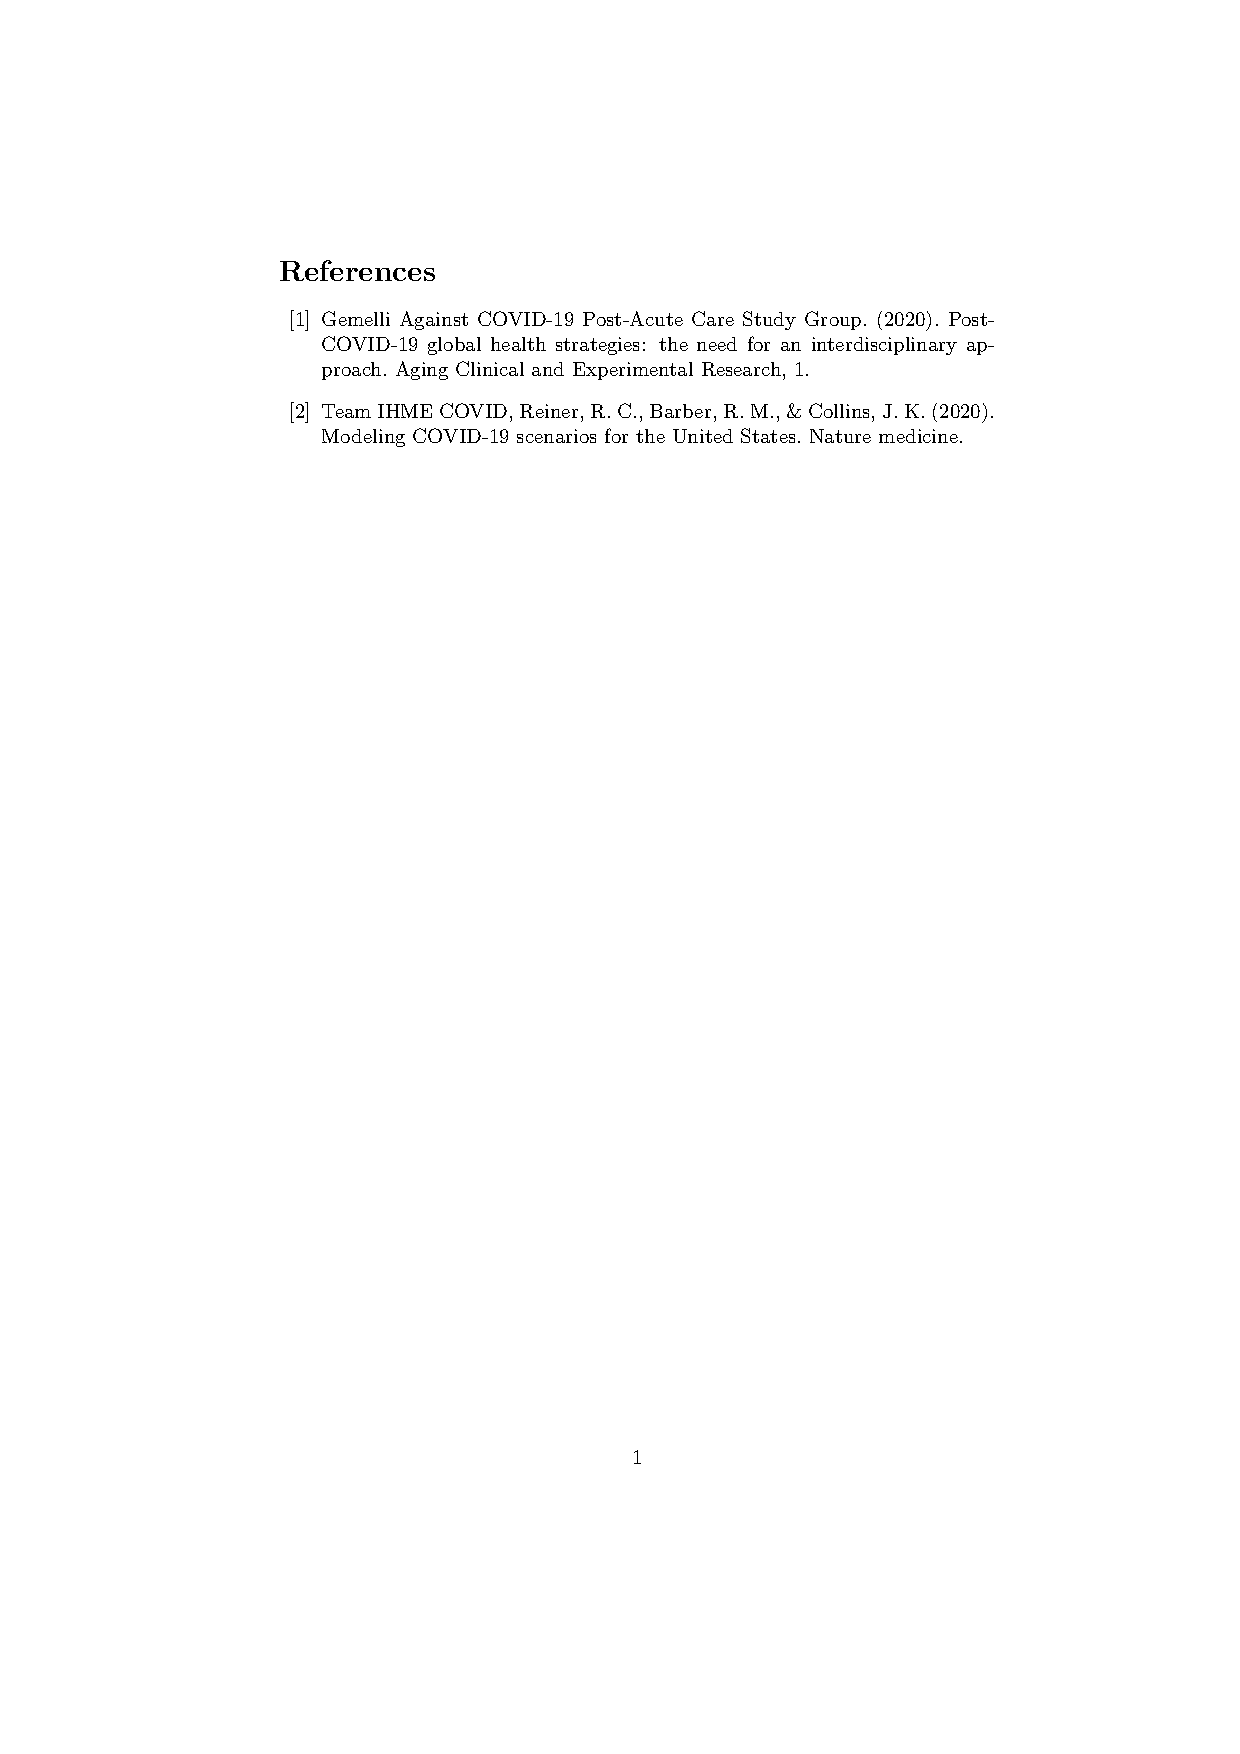
\includegraphics[width=\textwidth,trim={4cm 21.3cm 4cm 4cm},clip]{./pdf/ex6.pdf}
\end{framed}
\end{frame}

\begin{frame}[t, fragile]{참고문헌 목록}
		
	\tbs end\{document\} 위쪽(문서 끝자락)에 다음과 같이 thebibliography 환경을 만들고, bibitem 명령어로 문헌 정보를 기록한다.
	
\begin{block}{}	
	\begin{lstlisting}
\begin{thebibliography}{99}
\bibitem{gac2020} Gemelli Against COVID-19 Post-Acute Care Study Group. (2020). Post-COVID-19 global health strategies: the need for an interdisciplinary approach. Aging Clinical and Experimental Research, 1.

\bibitem{tic2020} Team IHME COVID, Reiner, R. C., Barber, R. M., \& Collins, J. K. (2020). Modeling COVID-19 scenarios for the United States. Nature medicine.
\end{thebibliography}
	\end{lstlisting}
\end{block}

\begin{itemize}
	\item 문헌의 label은 알파벳과 숫자로 구성하고, 알아보기 쉽게 저자+연도와 같이 적는 것이 편리하다.
	\item 문헌 정보를 적을 때에는 특수 문자 사용에 주의한다.		
\end{itemize}


\end{frame}


\begin{frame}[t, fragile]{참고문헌 표기 방식}
	
	2020년 R\&E 기준 표기 방식은 다음과 같다. 앞으로 올라올 R\&E 보고서 양식에 써 있는 표기 방식을 따르면 된다.
	
	\begin{framed}
		\centering
		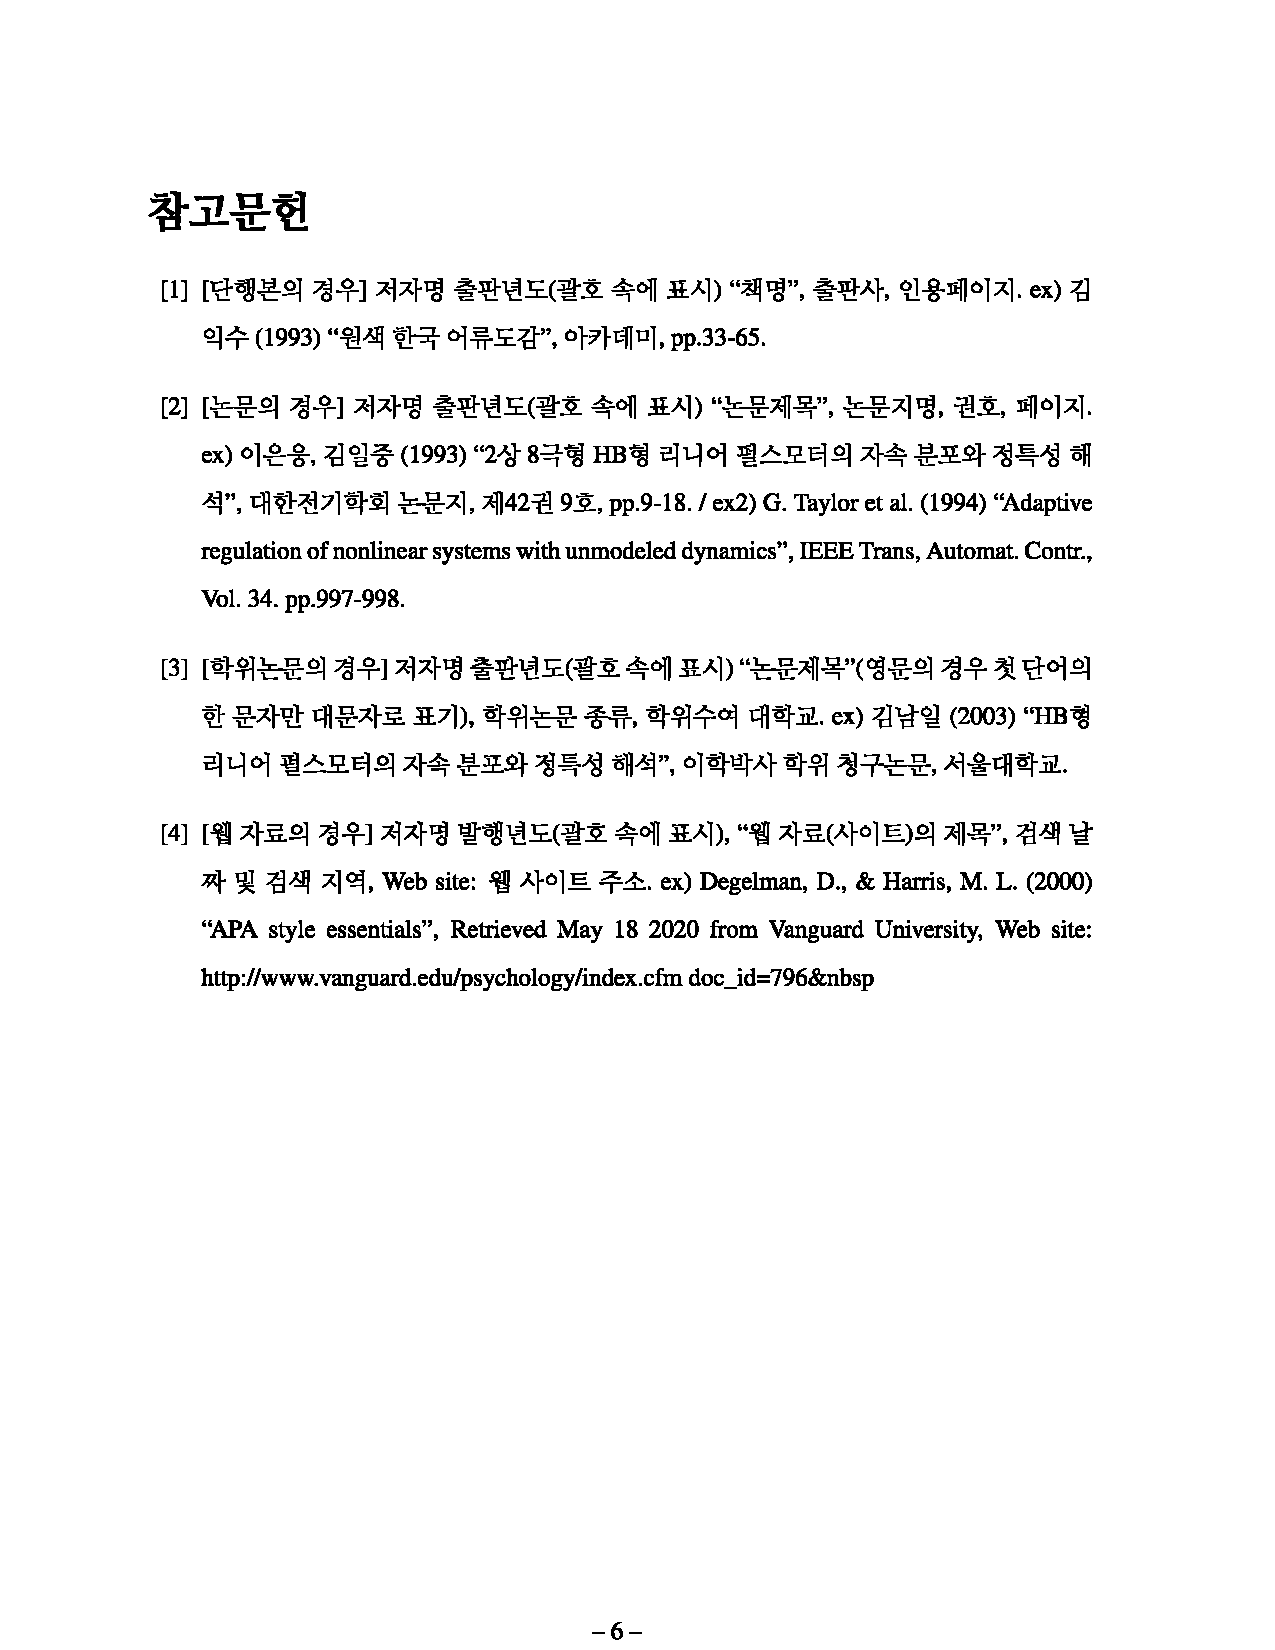
\includegraphics[width=.8\textwidth,trim={2.5cm 11cm 2.5cm 4.5cm},clip]{./pdf/bib.pdf}
	\end{framed}
	
	
\end{frame}

\begin{frame}[t, fragile]{참고문헌 인용}
	참고문헌을 본문에서 인용할 때는 \texttt{\tbs cite\{...\}}를 사용한다.
	\begin{itemize}
		\item \texttt{\tbs cite\{gac2020\}} $\rightarrow$ [1]
		\item \texttt{\tbs cite\{tic2020\}} $\rightarrow$ [2]
	\end{itemize}

\begin{block}{}
	\begin{lstlisting}
This paper is great\cite{gac2020}.
	\end{lstlisting}
\end{block}

\begin{framed}
	\textrm{This paper is great[1].}
\end{framed}
\end{frame}


\begin{frame}[t, fragile]{참조 및 인용 예시}
	
	\textbackslash \texttt{eqref\{ ... \} }, \textbackslash \texttt{ref\{ ... \} }, \textbackslash \texttt{cite\{ ... \} }은 참조와 인용에 사용되는 명령어이다. 보고서를 작성하기에 최적화된 명령어들이다!
	
	\begin{framed}
		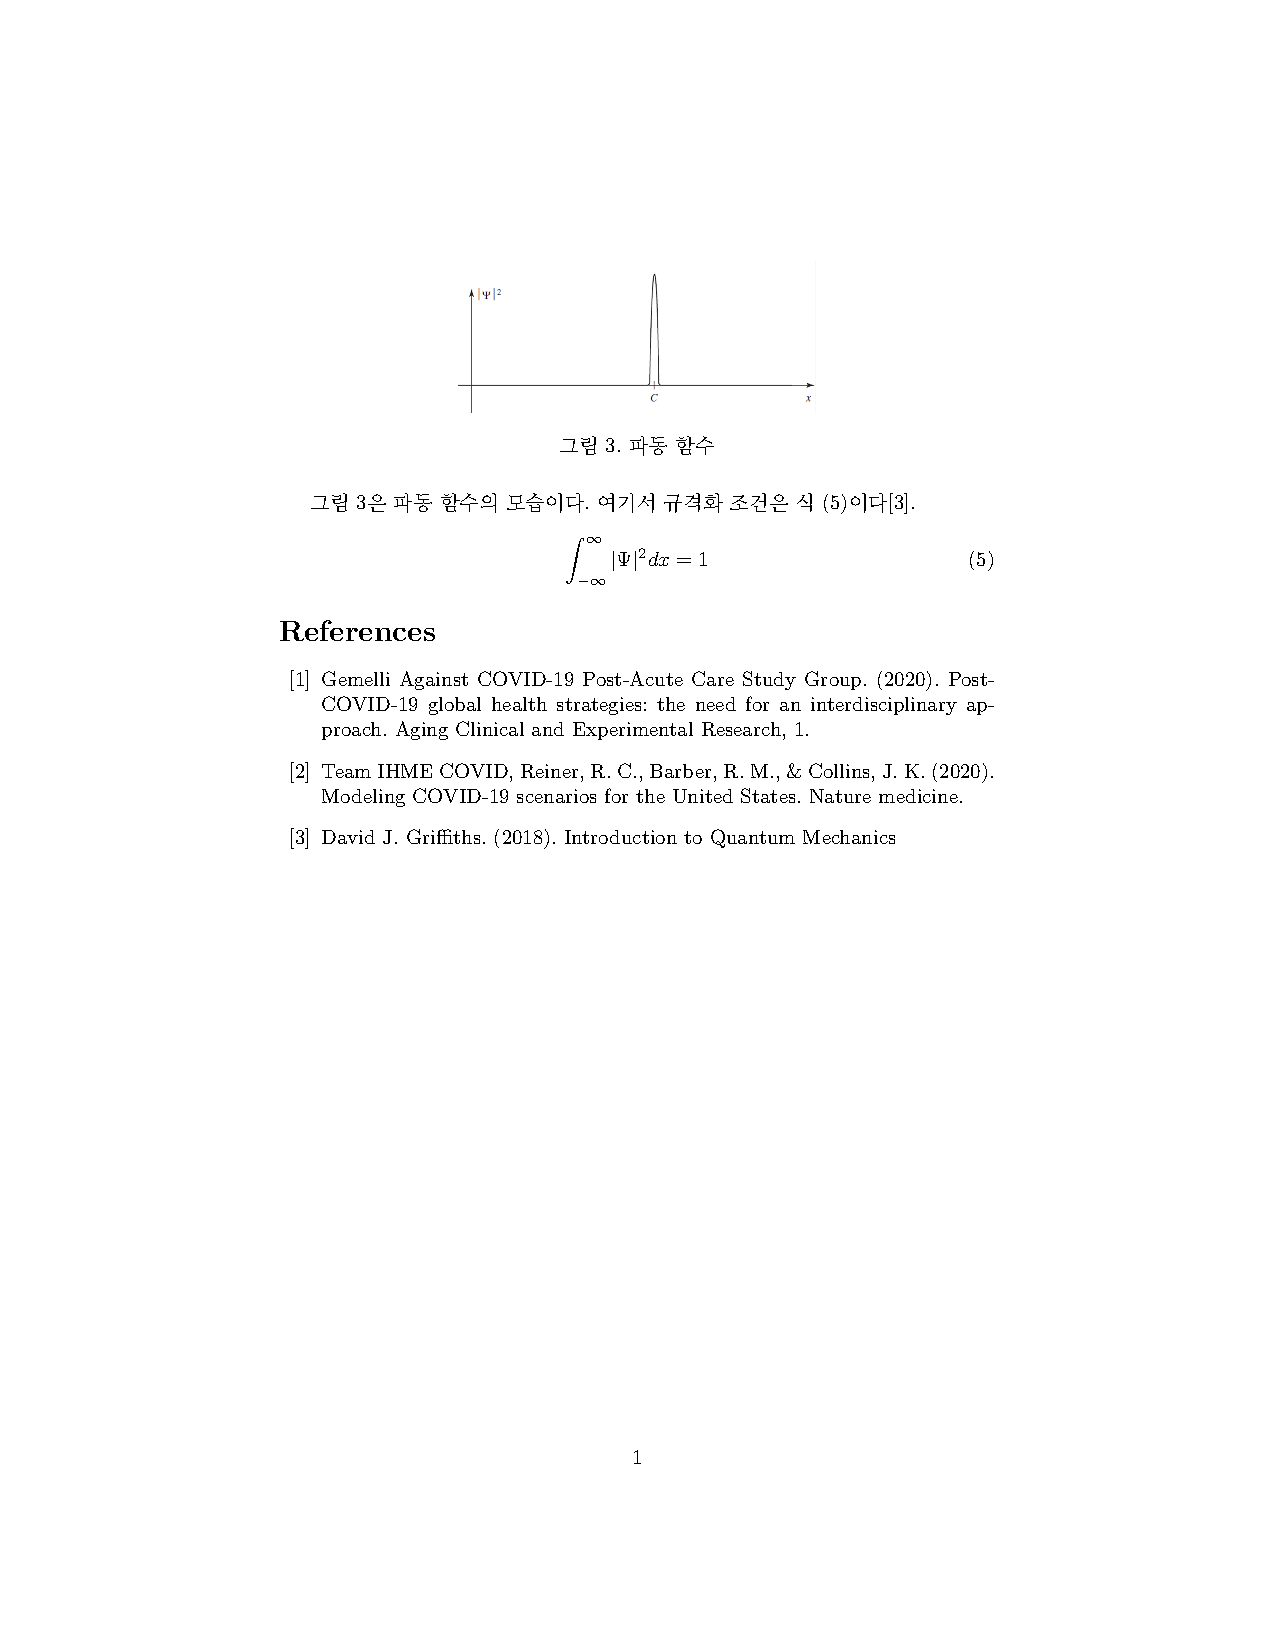
\includegraphics[width=\textwidth,trim={4cm 18cm 4cm 4cm},clip]{./pdf/refer1.pdf}
	\end{framed}
	
\end{frame}

\begin{frame}[t, fragile]{참조 및 인용 예시}
	
\begin{block}{}
\begin{lstlisting}
\begin{figure}[h]
	\centering
	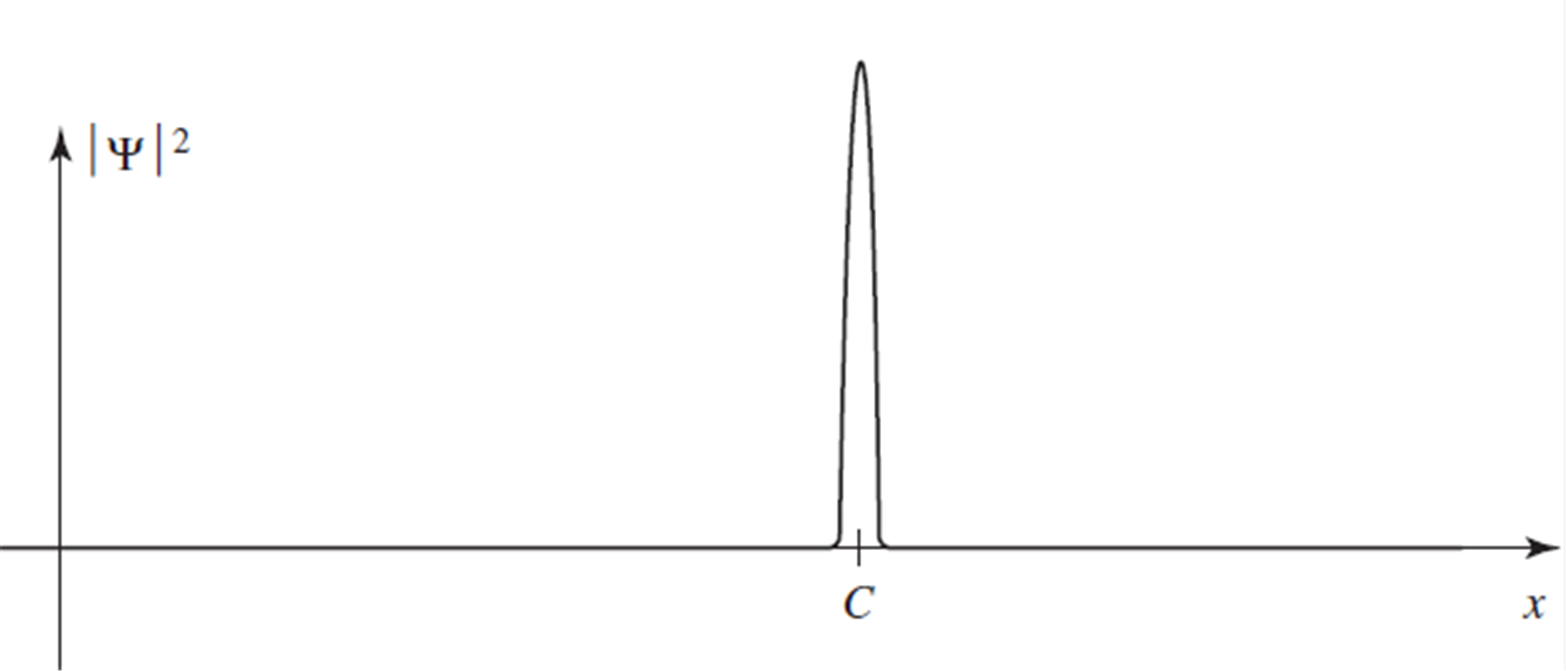
\includegraphics[width=0.5\textwidth]{wave_function.png}
	\caption{<@파동 함수@>}
	\label{fig:wave_function}
\end{figure}
<@그림@> \ref{fig:wave_function}<@은 파동 함수의 예시이다. 여기서 규격화 조건은 식@> \eqref{eq:normalization}<@이다@>\cite{griffiths2018}.
\begin{equation}
	\int_{-\infty}^{\infty} |\Psi|^2 dx = 1
	\label{eq:normalization}
\end{equation}
\end{lstlisting}
\end{block}
	
	
\end{frame}

\section{Remarks}
\subsection{Tips}

\begin{frame}[t]{Templates}
	\begin{itemize}
		\item 지금까지는 \LaTeX{}에서 제공한 기본 형식에 맞춰 문서를 만들었다.
		\item 그러나 문서를 작성하다 보면 형식을 바꿔야 하는 일이 생긴다.
		\begin{itemize}
			\item 나만의 스타일로 문서를 만들고 싶은 경우
			\item 논문, 보고서 등 형식이 정해진 문서를 만드는 경우
		\end{itemize}
		\item 본인이 직접 문서 스타일을 설정할 수 있으나 복잡하고 어렵다.
		\item 이때 남이 만들어둔 템플릿이 있다면 그 템플릿을 그대로 받아 사용하면 된다.
	\end{itemize}
\end{frame}

\begin{frame}[t]{GSHS Format}
	
	경기과학고 \TeX{} 협회에서는 경곽 학생들이 사용할 수 있는 다양한 문서 템플릿들을 제공한다. \footnotesize $\rightarrow$ 휴먼테크 논문대상, 경기과학고 Beamer\footnote[frame]{이 문서는 gshs\_beamer\_ver2 템플릿으로 제작되었다.}, R\&E 연구 보고서, R\&E 포스터, (졸업논문) ...
	
	\vspace{20pt}
	
	\small \textbf{URL:} \url{https://github.com/gshslatexintro/gshs-format}
		\begin{figure}[h]
			\centering
			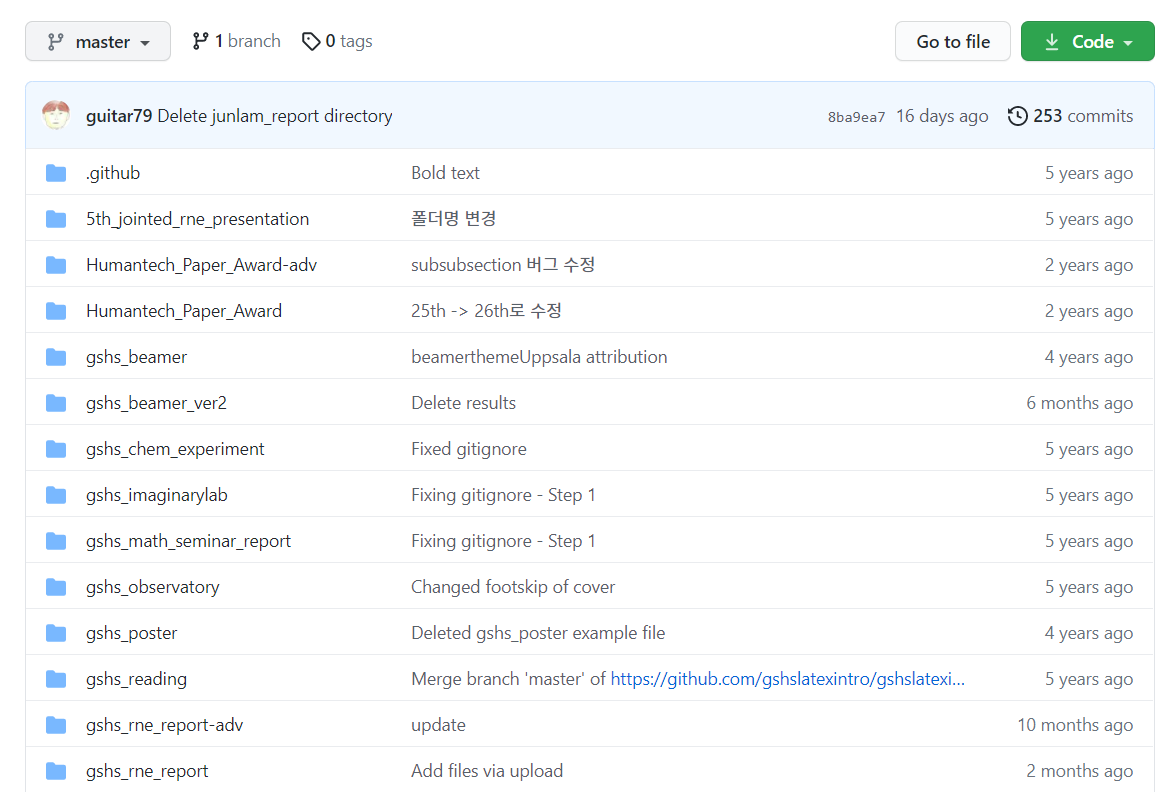
\includegraphics[width=.6\textwidth]{./figures/latexgshs.png}
		\end{figure}
	
\end{frame}

\begin{frame}[t]{R\&E 보고서 양식}

		\url{https://github.com/gshslatexintro/gshs-format/tree/master/gshs_rne_report}
		\begin{figure}[h]
			\centering
			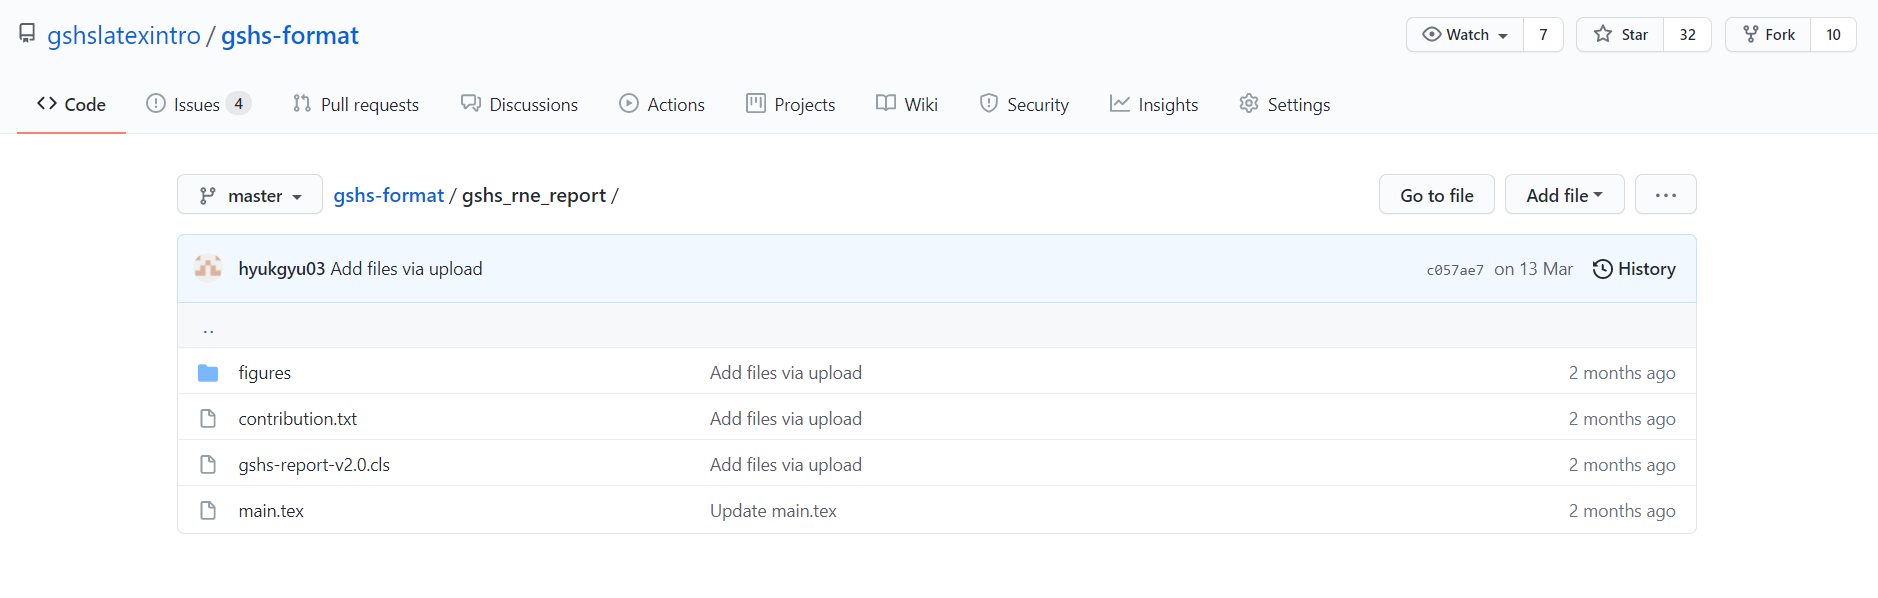
\includegraphics[width=\textwidth]{./figures/latexgshs_rne.png}
		\end{figure}
	
	Fork 기능을 이용하면 다운로드가 가능하다. 그러나 Github 사용법에 익숙치 않은 사람들을 위해 `송죽학사 $>$ 게시판 $>$ 자유게시판'에도 양식을 업로드하였다.

\end{frame}

\begin{frame}[t]{Tips}
1) \Large \color{red} \textbf{Ask Google!} \color{black} \small --- 모르는 건 Google에게
\begin{itemize}
	\item \textbf{Q1.} 글자 크기는 어떻게 바꿔요?
	$\rightarrow$ latex font size changing
	\item \textbf{Q2.} itemize 줄간격 어떻게 바꾸죠? $\rightarrow$ latex itemize line spacing
	\item 키워드를 모르겠다면, 횡설수설 검색하다가 키워드를 찾고, 그 키워드로 다시 검색한다.
\end{itemize}
\vspace{12pt}
2) 컴파일 에러
\begin{itemize}
	\item 한번에 너무 많은 코드를 추가하면 컴파일 에러 원인 찾기 어려움! 중간중간에 컴파일하기
	\item 환경에서 begin-end 쌍 안 맞음, 중괄호 \{ \} 개수 다름, 특수 문자 입력 실수 등 문법 오류
	\item 잘 모르겠다면, 에러 메시지를 복사해서 검색
	\item 과학적 사고. 조금씩 주석처리하면서 문제되는 부분 탐색 $\rightarrow$ 최소 작동 예시 (minimal working example)
\end{itemize}
\end{frame}

\begin{frame}[t]{Further Tips}
	
	3) 자주 사용해야 하는 긴 명령어가 있는 경우 \texttt{\tbs newcommand} 명령어를 통해 짧은 명령어로 바꿔 사용할 수 있다.
	
	\vspace{15pt}
	4) \texttt{\tbs newenvironment}를 통해 새로운 환경을 정의하고 사용할 수 있다.
	
	\vspace{15pt}
	5) 클래스 파일(*.cls)을 만들면 새로운 문서 서식을 정의하여 사용할 수 있다.

\end{frame}


\subsection{GSHS \TeX{} Society}

\begin{frame}[t]{경기과학고 \TeX{} 사용자 협회}
	\textbf{Homepage:} \url{http://latex.gs.hs.kr/}
	\begin{figure}[h]
		\centering
		
\includegraphics[width=.7\textwidth]{./figures/texcoop.png}
	\end{figure}

	다른 소통 창구
	\begin{itemize}
		\item \textbf{Facebook:} 경기과학고 \TeX 사용자 협회 페이지
		\item \textbf{Github:} \url{https://github.com/gshslatexintro} (e-mail 有)
		
	\end{itemize}
\end{frame}

\begin{frame}[t]{경기과학고 \TeX{} 사용자 협회}
	
	\textbf{소개}
	\begin{itemize}
		\item 2015.08.02 설립 (32기 박승원)
		\item \TeX{}에 관심 있는 경기과학고 학생 $\cdot$ 교사들의 협회
		\item ``\TeX 사용 진입 장벽을 없애고, 양식 파일을 만들자!''
	\end{itemize}
	
	\vspace{20pt}
	\textbf{하는 일}
	\begin{itemize}
		\item 교내 관련 \LaTeX{} 양식 제작 및 배포 (Github)
		\item \LaTeX \ 입문서 편찬 (現 중단)
		\item Workshop 개최
	\end{itemize}

\vspace{20pt}
$\Rightarrow$ \TeX{}에 관심 있는 경기과학고 재학생/교원이라면 누구나 참여 가능
\end{frame}

\begin{frame}[t]{협회 참여}
	
	\textbf{참여 방법}
	\begin{enumerate}
		\item Github 회원 가입: 주로 Github를 통해 협회 활동이 진행되니, 기본적인 Github 사용법을 알아두시기를 권장합니다.
		\item 참여 신청 (3가지 중 택 1)
		\begin{itemize}
			\item Facebook의 \TeX{} 협회 페이지로 참여 메시지 전송
			\item Github의 e-mail 주소로 참여 메시지 전송
			\item 박기현 선생님께 직접 말씀 드려도 됩니다.
		\end{itemize}
	\end{enumerate}

	\vspace{15pt}
	협회 활동은 \TeX 을 누구보다 체계적으로 공부해볼 수 있는 절호의 기회입니다! 2022년을 이끌어갈 38기 회장, 부회장, 웹마스터도 모집.
	
	\vspace{15pt}
	지난해 COVID-19로 인해 학년간 교류가 거의 이루어지지 않아 \TeX{}협회에는 38기가 없는 상황입니다. 38, 39기 학생 여러분의 많은 관심 부탁드립니다.
	
\end{frame}

\subsection{}

\begin{frame}[t]{끝}
	감사합니다.
	\vspace{15pt}
	
	Special Thanks to...
	
	\begin{itemize}
		\item 박기현 선생님
		\item 37기 한수민
		\item 35기 \TeX \ 사용자 협회
	\end{itemize}
\end{frame}

\end{document}